\documentclass[twoside]{book}

% Packages required by doxygen
\usepackage{fixltx2e}
\usepackage{calc}
\usepackage{doxygen}
\usepackage[export]{adjustbox} % also loads graphicx
\usepackage{graphicx}
\usepackage[utf8]{inputenc}
\usepackage{makeidx}
\usepackage{multicol}
\usepackage{multirow}
\PassOptionsToPackage{warn}{textcomp}
\usepackage{textcomp}
\usepackage[nointegrals]{wasysym}
\usepackage[table]{xcolor}

% Font selection
\usepackage[T1]{fontenc}
\usepackage[scaled=.90]{helvet}
\usepackage{courier}
\usepackage{amssymb}
\usepackage{sectsty}
\renewcommand{\familydefault}{\sfdefault}
\allsectionsfont{%
  \fontseries{bc}\selectfont%
  \color{darkgray}%
}
\renewcommand{\DoxyLabelFont}{%
  \fontseries{bc}\selectfont%
  \color{darkgray}%
}
\newcommand{\+}{\discretionary{\mbox{\scriptsize$\hookleftarrow$}}{}{}}

% Page & text layout
\usepackage{geometry}
\geometry{%
  a4paper,%
  top=2.5cm,%
  bottom=2.5cm,%
  left=2.5cm,%
  right=2.5cm%
}
\tolerance=750
\hfuzz=15pt
\hbadness=750
\setlength{\emergencystretch}{15pt}
\setlength{\parindent}{0cm}
\setlength{\parskip}{3ex plus 2ex minus 2ex}
\makeatletter
\renewcommand{\paragraph}{%
  \@startsection{paragraph}{4}{0ex}{-1.0ex}{1.0ex}{%
    \normalfont\normalsize\bfseries\SS@parafont%
  }%
}
\renewcommand{\subparagraph}{%
  \@startsection{subparagraph}{5}{0ex}{-1.0ex}{1.0ex}{%
    \normalfont\normalsize\bfseries\SS@subparafont%
  }%
}
\makeatother

% Headers & footers
\usepackage{fancyhdr}
\pagestyle{fancyplain}
\fancyhead[LE]{\fancyplain{}{\bfseries\thepage}}
\fancyhead[CE]{\fancyplain{}{}}
\fancyhead[RE]{\fancyplain{}{\bfseries\leftmark}}
\fancyhead[LO]{\fancyplain{}{\bfseries\rightmark}}
\fancyhead[CO]{\fancyplain{}{}}
\fancyhead[RO]{\fancyplain{}{\bfseries\thepage}}
\fancyfoot[LE]{\fancyplain{}{}}
\fancyfoot[CE]{\fancyplain{}{}}
\fancyfoot[RE]{\fancyplain{}{\bfseries\scriptsize 制作者 Doxygen }}
\fancyfoot[LO]{\fancyplain{}{\bfseries\scriptsize 制作者 Doxygen }}
\fancyfoot[CO]{\fancyplain{}{}}
\fancyfoot[RO]{\fancyplain{}{}}
\renewcommand{\footrulewidth}{0.4pt}
\renewcommand{\chaptermark}[1]{%
  \markboth{#1}{}%
}
\renewcommand{\sectionmark}[1]{%
  \markright{\thesection\ #1}%
}

% Indices & bibliography
\usepackage{natbib}
\usepackage[titles]{tocloft}
\setcounter{tocdepth}{3}
\setcounter{secnumdepth}{5}
\makeindex

% Hyperlinks (required, but should be loaded last)
\usepackage{ifpdf}
\ifpdf
  \usepackage[pdftex,pagebackref=true]{hyperref}
\else
  \usepackage[ps2pdf,pagebackref=true]{hyperref}
\fi
\hypersetup{%
  colorlinks=true,%
  linkcolor=blue,%
  citecolor=blue,%
  unicode%
}

% Custom commands
\newcommand{\clearemptydoublepage}{%
  \newpage{\pagestyle{empty}\cleardoublepage}%
}

\usepackage{caption}
\captionsetup{labelsep=space,justification=centering,font={bf},singlelinecheck=off,skip=4pt,position=top}

%===== C O N T E N T S =====

\begin{document}

% Titlepage & ToC
\hypersetup{pageanchor=false,
             bookmarksnumbered=true,
             pdfencoding=unicode
            }
\pagenumbering{alph}
\begin{titlepage}
\vspace*{7cm}
\begin{center}%
{\Large C\+C\+\_\+\+P\+L\+A\+Y\+\_\+\+S\+D\+K\+\_\+\+A\+PI }\\
\vspace*{1cm}
{\large 制作者 Doxygen 1.8.13}\\
\end{center}
\end{titlepage}
\clearemptydoublepage
\pagenumbering{roman}
\tableofcontents
\clearemptydoublepage
\pagenumbering{arabic}
\hypersetup{pageanchor=true}

%--- Begin generated contents ---
\chapter{继承关系索引}
\section{类继承关系}
此继承关系列表按字典顺序粗略的排序\+: \begin{DoxyCompactList}
\item N\+S\+Object\begin{DoxyCompactList}
\item \contentsline{section}{Offline\+Play\+Back}{\pageref{interface_offline_play_back}}{}
\item \contentsline{section}{Play\+Parameter}{\pageref{interface_play_parameter}}{}
\item \contentsline{section}{Request\+Data}{\pageref{interface_request_data}}{}
\item \contentsline{section}{Request\+Data\+Play\+Back}{\pageref{interface_request_data_play_back}}{}
\item \contentsline{section}{Save\+Log\+Util}{\pageref{interface_save_log_util}}{}
\end{DoxyCompactList}
\item $<$N\+S\+Object$>$\begin{DoxyCompactList}
\item \contentsline{section}{$<$Offline\+Play\+Back\+Delegate $>$}{\pageref{protocol_offline_play_back_delegate_01-p}}{}
\item \contentsline{section}{$<$Request\+Data\+Delegate $>$}{\pageref{protocol_request_data_delegate_01-p}}{}
\item \contentsline{section}{$<$Request\+Data\+Play\+Back\+Delegate $>$}{\pageref{protocol_request_data_play_back_delegate_01-p}}{}
\end{DoxyCompactList}
\end{DoxyCompactList}

\chapter{类索引}
\section{类列表}
这里列出了所有类、结构、联合以及接口定义等,并附带简要说明\+:\begin{DoxyCompactList}
\item\contentsline{section}{\hyperlink{interface_offline_play_back}{Offline\+Play\+Back} }{\pageref{interface_offline_play_back}}{}
\item\contentsline{section}{\hyperlink{protocol_offline_play_back_delegate_01-p}{$<$\+Offline\+Play\+Back\+Delegate $>$} }{\pageref{protocol_offline_play_back_delegate_01-p}}{}
\item\contentsline{section}{\hyperlink{interface_play_parameter}{Play\+Parameter} }{\pageref{interface_play_parameter}}{}
\item\contentsline{section}{\hyperlink{interface_request_data}{Request\+Data} }{\pageref{interface_request_data}}{}
\item\contentsline{section}{\hyperlink{protocol_request_data_delegate_01-p}{$<$\+Request\+Data\+Delegate $>$} }{\pageref{protocol_request_data_delegate_01-p}}{}
\item\contentsline{section}{\hyperlink{interface_request_data_play_back}{Request\+Data\+Play\+Back} }{\pageref{interface_request_data_play_back}}{}
\item\contentsline{section}{\hyperlink{protocol_request_data_play_back_delegate_01-p}{$<$\+Request\+Data\+Play\+Back\+Delegate $>$} }{\pageref{protocol_request_data_play_back_delegate_01-p}}{}
\item\contentsline{section}{\hyperlink{interface_save_log_util}{Save\+Log\+Util} }{\pageref{interface_save_log_util}}{}
\end{DoxyCompactList}

\chapter{类说明}
\hypertarget{interface_offline_play_back}{}\section{Offline\+Play\+Back类 参考}
\label{interface_offline_play_back}\index{Offline\+Play\+Back@{Offline\+Play\+Back}}
类 Offline\+Play\+Back 继承关系图\+:\begin{figure}[H]
\begin{center}
\leavevmode
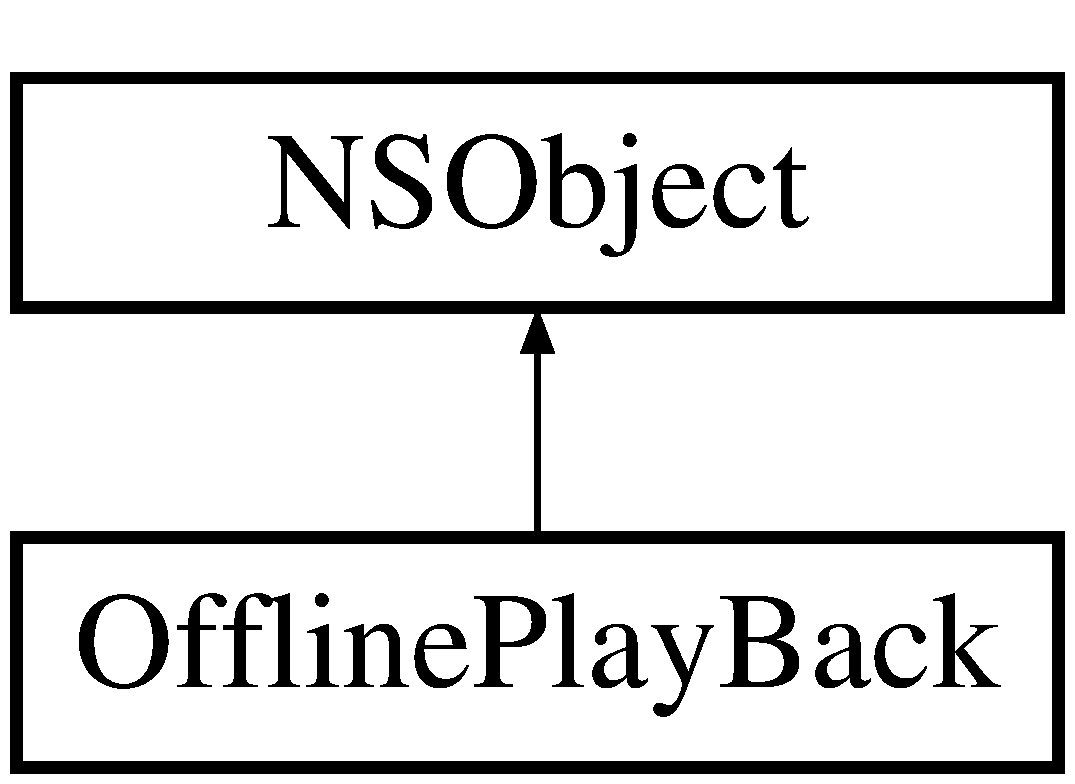
\includegraphics[height=2.000000cm]{interface_offline_play_back}
\end{center}
\end{figure}
\subsection*{构造函数}
\begin{DoxyCompactItemize}
\item 
(id) -\/ \hyperlink{interface_offline_play_back_af03e324fc6ecf88ef231c945de5b1a5c}{init\+With\+Parameter\+:}
\begin{DoxyCompactList}\small\item\em 初始化 \end{DoxyCompactList}\item 
\mbox{\Hypertarget{interface_offline_play_back_a066a30821438528546ac1f4ed205975d}\label{interface_offline_play_back_a066a30821438528546ac1f4ed205975d}} 
(void) -\/ \hyperlink{interface_offline_play_back_a066a30821438528546ac1f4ed205975d}{start\+Play\+And\+Decompress}
\begin{DoxyCompactList}\small\item\em 开始解析数据并播放视频 \end{DoxyCompactList}\item 
\mbox{\Hypertarget{interface_offline_play_back_a7b71e7e41545db196953fe6bc3462b35}\label{interface_offline_play_back_a7b71e7e41545db196953fe6bc3462b35}} 
(void) -\/ \hyperlink{interface_offline_play_back_a7b71e7e41545db196953fe6bc3462b35}{request\+Cancel}
\begin{DoxyCompactList}\small\item\em 销毁文档和视频,清除视频和文档的时候需要调用,推出播放页面的时候也需要调用 \end{DoxyCompactList}\item 
\mbox{\Hypertarget{interface_offline_play_back_a8078e7716f7c41146c094b6fd637c924}\label{interface_offline_play_back_a8078e7716f7c41146c094b6fd637c924}} 
(void) -\/ \hyperlink{interface_offline_play_back_a8078e7716f7c41146c094b6fd637c924}{continue\+From\+The\+Time\+:}
\begin{DoxyCompactList}\small\item\em time:从直播开始到现在的秒数,\+S\+D\+K会在画板上绘画出来相应的图形 \end{DoxyCompactList}\item 
\mbox{\Hypertarget{interface_offline_play_back_aa9822fbb0c3958a1ac4cb9fd48cc5450}\label{interface_offline_play_back_aa9822fbb0c3958a1ac4cb9fd48cc5450}} 
(C\+G\+Float) -\/ \hyperlink{interface_offline_play_back_aa9822fbb0c3958a1ac4cb9fd48cc5450}{get\+Doc\+Aspect\+Ratio}
\begin{DoxyCompactList}\small\item\em 获取文档区域内白板或者文档本身的宽高比,返回值即为宽高比,做屏幕适配用 \end{DoxyCompactList}\item 
\mbox{\Hypertarget{interface_offline_play_back_a62d3c2f0558f3ce002251dd98e84dbcf}\label{interface_offline_play_back_a62d3c2f0558f3ce002251dd98e84dbcf}} 
(void) -\/ \hyperlink{interface_offline_play_back_a62d3c2f0558f3ce002251dd98e84dbcf}{change\+Doc\+Frame\+:}
\begin{DoxyCompactList}\small\item\em 改变文档区域大小,主要用在文档生成后改变文档窗口的frame \end{DoxyCompactList}\item 
\mbox{\Hypertarget{interface_offline_play_back_ac1c40aab1bea6b80a33292a0cfddf002}\label{interface_offline_play_back_ac1c40aab1bea6b80a33292a0cfddf002}} 
(void) -\/ \hyperlink{interface_offline_play_back_ac1c40aab1bea6b80a33292a0cfddf002}{change\+Player\+Frame\+:}
\begin{DoxyCompactList}\small\item\em 改变播放器frame \end{DoxyCompactList}\item 
\mbox{\Hypertarget{interface_offline_play_back_ae83e564798be358b00fb6b0e7172d0f8}\label{interface_offline_play_back_ae83e564798be358b00fb6b0e7172d0f8}} 
(void) -\/ \hyperlink{interface_offline_play_back_ae83e564798be358b00fb6b0e7172d0f8}{change\+Player\+Parent\+:}
\begin{DoxyCompactList}\small\item\em 改变播放器父窗口 \end{DoxyCompactList}\item 
\mbox{\Hypertarget{interface_offline_play_back_ae90886ca0199a300d123b8dfee178a47}\label{interface_offline_play_back_ae90886ca0199a300d123b8dfee178a47}} 
(void) -\/ \hyperlink{interface_offline_play_back_ae90886ca0199a300d123b8dfee178a47}{change\+Doc\+Parent\+:}
\begin{DoxyCompactList}\small\item\em 改变文档父窗口 \end{DoxyCompactList}\item 
\mbox{\Hypertarget{interface_offline_play_back_afe2a5924e708c918515133b9ded58789}\label{interface_offline_play_back_afe2a5924e708c918515133b9ded58789}} 
(void) -\/ \hyperlink{interface_offline_play_back_afe2a5924e708c918515133b9ded58789}{pause\+Player}
\begin{DoxyCompactList}\small\item\em 播放器暂停 \end{DoxyCompactList}\item 
\mbox{\Hypertarget{interface_offline_play_back_a96d5cf73bdffcd575a2e5100547e6e91}\label{interface_offline_play_back_a96d5cf73bdffcd575a2e5100547e6e91}} 
(void) -\/ \hyperlink{interface_offline_play_back_a96d5cf73bdffcd575a2e5100547e6e91}{start\+Player}
\begin{DoxyCompactList}\small\item\em 播放器播放 \end{DoxyCompactList}\item 
\mbox{\Hypertarget{interface_offline_play_back_ae9a74cc8b04aec15c364fb2a61a2fee9}\label{interface_offline_play_back_ae9a74cc8b04aec15c364fb2a61a2fee9}} 
(void) -\/ \hyperlink{interface_offline_play_back_ae9a74cc8b04aec15c364fb2a61a2fee9}{shutdown\+Player}
\begin{DoxyCompactList}\small\item\em 播放器关闭并移除 \end{DoxyCompactList}\item 
\mbox{\Hypertarget{interface_offline_play_back_a7dde7a57cc513fb9ebb3e5e635e0eb9a}\label{interface_offline_play_back_a7dde7a57cc513fb9ebb3e5e635e0eb9a}} 
(void) -\/ \hyperlink{interface_offline_play_back_a7dde7a57cc513fb9ebb3e5e635e0eb9a}{stop\+Player}
\begin{DoxyCompactList}\small\item\em 播放器停止 \end{DoxyCompactList}\item 
\mbox{\Hypertarget{interface_offline_play_back_a048137f526fa9e1305441ebac3833cd7}\label{interface_offline_play_back_a048137f526fa9e1305441ebac3833cd7}} 
(void) -\/ \hyperlink{interface_offline_play_back_a048137f526fa9e1305441ebac3833cd7}{replay\+Player}
\begin{DoxyCompactList}\small\item\em 从头播放 \end{DoxyCompactList}\item 
\mbox{\Hypertarget{interface_offline_play_back_a86f033aa94f7532be970bea92076af31}\label{interface_offline_play_back_a86f033aa94f7532be970bea92076af31}} 
(B\+O\+OL) -\/ \hyperlink{interface_offline_play_back_a86f033aa94f7532be970bea92076af31}{is\+Playing}
\begin{DoxyCompactList}\small\item\em 播放器是否播放 \end{DoxyCompactList}\item 
\mbox{\Hypertarget{interface_offline_play_back_ab19a16ddbca9ee34085ce5250aaf02ee}\label{interface_offline_play_back_ab19a16ddbca9ee34085ce5250aaf02ee}} 
(N\+S\+Time\+Interval) -\/ \hyperlink{interface_offline_play_back_ab19a16ddbca9ee34085ce5250aaf02ee}{current\+Playback\+Time}
\begin{DoxyCompactList}\small\item\em 播放器当前播放时间 \end{DoxyCompactList}\item 
\mbox{\Hypertarget{interface_offline_play_back_a5073e3c5fa97621523a5a6a3b8163238}\label{interface_offline_play_back_a5073e3c5fa97621523a5a6a3b8163238}} 
(void) -\/ \hyperlink{interface_offline_play_back_a5073e3c5fa97621523a5a6a3b8163238}{set\+Current\+Playback\+Time\+:}
\begin{DoxyCompactList}\small\item\em 设置播放器当前播放时间(用于拖拽进度条时掉用的) \end{DoxyCompactList}\item 
\mbox{\Hypertarget{interface_offline_play_back_acf85129c9552cbe05a4b925199385d32}\label{interface_offline_play_back_acf85129c9552cbe05a4b925199385d32}} 
(N\+S\+Time\+Interval) -\/ \hyperlink{interface_offline_play_back_acf85129c9552cbe05a4b925199385d32}{player\+Duration}
\begin{DoxyCompactList}\small\item\em 回放视频总时长 \end{DoxyCompactList}\item 
\mbox{\Hypertarget{interface_offline_play_back_aecc8a54b8b74b3b34e28d9d341b4dac1}\label{interface_offline_play_back_aecc8a54b8b74b3b34e28d9d341b4dac1}} 
(void) -\/ \hyperlink{interface_offline_play_back_aecc8a54b8b74b3b34e28d9d341b4dac1}{setpause\+In\+Back\+Ground\+:}
\begin{DoxyCompactList}\small\item\em 设置后台是否可播放 \end{DoxyCompactList}\end{DoxyCompactItemize}
\subsection*{属性}
\begin{DoxyCompactItemize}
\item 
\mbox{\Hypertarget{interface_offline_play_back_a27b124ec76c47345b93524a6bfd321e2}\label{interface_offline_play_back_a27b124ec76c47345b93524a6bfd321e2}} 
id$<$ Offline\+Play\+Back\+Delegate $>$ \hyperlink{interface_offline_play_back_a27b124ec76c47345b93524a6bfd321e2}{delegate}
\begin{DoxyCompactList}\small\item\em 代理 \end{DoxyCompactList}\item 
\mbox{\Hypertarget{interface_offline_play_back_a67fb8ebdc8ff25d7fd9feeb028b4432b}\label{interface_offline_play_back_a67fb8ebdc8ff25d7fd9feeb028b4432b}} 
id$<$ I\+J\+K\+Media\+Playback $>$ \hyperlink{interface_offline_play_back_a67fb8ebdc8ff25d7fd9feeb028b4432b}{ijk\+Player}
\begin{DoxyCompactList}\small\item\em 播放器 \end{DoxyCompactList}\end{DoxyCompactItemize}


\subsection{函数文档}
\mbox{\Hypertarget{interface_offline_play_back_af03e324fc6ecf88ef231c945de5b1a5c}\label{interface_offline_play_back_af03e324fc6ecf88ef231c945de5b1a5c}} 
\index{Offline\+Play\+Back@{Offline\+Play\+Back}!init\+With\+Parameter\+:@{init\+With\+Parameter\+:}}
\index{init\+With\+Parameter\+:@{init\+With\+Parameter\+:}!Offline\+Play\+Back@{Offline\+Play\+Back}}
\subsubsection{\texorpdfstring{init\+With\+Parameter\+:()}{initWithParameter:()}}
{\footnotesize\ttfamily -\/ (id) init\+With\+Parameter\+: \begin{DoxyParamCaption}\item[{(\hyperlink{interface_play_parameter}{Play\+Parameter} $\ast$)}]{parameter }\end{DoxyParamCaption}}



初始化 


\begin{DoxyParams}{参数}
{\em parameter} & 配置参数信息 必填参数 doc\+Frame; 必填参数 doc\+Parent; 必填参数 player\+Parent; 必填参数 player\+Frame; 必填参数 scaling\+Mode; 必填参数 destination; 必填参数 default\+Color; 必填参数 P\+P\+T\+Scaling\+Mode; 必填参数 pause\+In\+Back\+Ground; \\
\hline
\end{DoxyParams}


该类的文档由以下文件生成\+:\begin{DoxyCompactItemize}
\item 
Offline\+Play\+Back.\+h\end{DoxyCompactItemize}

\hypertarget{protocol_offline_play_back_delegate_01-p}{}\section{$<$Offline\+Play\+Back\+Delegate $>$协议 参考}
\label{protocol_offline_play_back_delegate_01-p}\index{$<$\+Offline\+Play\+Back\+Delegate $>$@{$<$\+Offline\+Play\+Back\+Delegate $>$}}
类 $<$Offline\+Play\+Back\+Delegate $>$ 继承关系图\+:\begin{figure}[H]
\begin{center}
\leavevmode
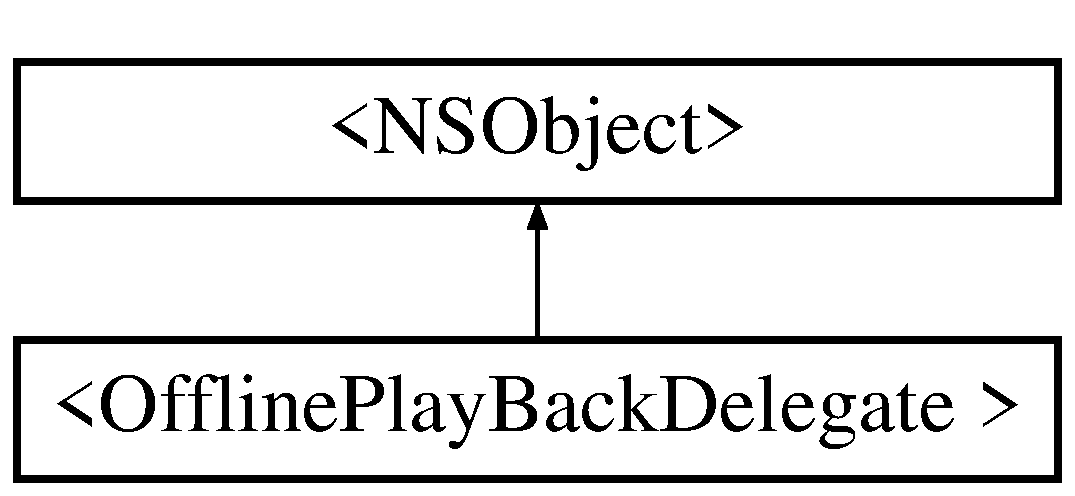
\includegraphics[height=2.000000cm]{protocol_offline_play_back_delegate_01-p}
\end{center}
\end{figure}
\subsection*{构造函数}
\begin{DoxyCompactItemize}
\item 
\mbox{\Hypertarget{protocol_offline_play_back_delegate_01-p_a1ee776037831d9c6f44a635f19be821a}\label{protocol_offline_play_back_delegate_01-p_a1ee776037831d9c6f44a635f19be821a}} 
(void) -\/ \hyperlink{protocol_offline_play_back_delegate_01-p_a1ee776037831d9c6f44a635f19be821a}{offline\+\_\+get\+Doc\+Aspect\+Ratio\+Of\+Width\+:height\+:}
\begin{DoxyCompactList}\small\item\em 获取文档内白板或者文档本身的宽高,来进行屏幕适配用的 \end{DoxyCompactList}\item 
\mbox{\Hypertarget{protocol_offline_play_back_delegate_01-p_a4a95cda1929dc7cb1ed2b248a7542d38}\label{protocol_offline_play_back_delegate_01-p_a4a95cda1929dc7cb1ed2b248a7542d38}} 
(void) -\/ \hyperlink{protocol_offline_play_back_delegate_01-p_a4a95cda1929dc7cb1ed2b248a7542d38}{offline\+\_\+on\+Parser\+Question\+Arr\+:on\+Parser\+Answer\+Arr\+:}
\begin{DoxyCompactList}\small\item\em 收到本房间的历史提问\&回答 \end{DoxyCompactList}\item 
\mbox{\Hypertarget{protocol_offline_play_back_delegate_01-p_abb9d5988a67cf4cdc583d1782709146f}\label{protocol_offline_play_back_delegate_01-p_abb9d5988a67cf4cdc583d1782709146f}} 
(void) -\/ \hyperlink{protocol_offline_play_back_delegate_01-p_abb9d5988a67cf4cdc583d1782709146f}{offline\+\_\+on\+Parser\+Chat\+:}
\begin{DoxyCompactList}\small\item\em 解析本房间的历史聊天数据 \end{DoxyCompactList}\item 
\mbox{\Hypertarget{protocol_offline_play_back_delegate_01-p_a89a33f4e08be57b1019c80f508bf2bb0}\label{protocol_offline_play_back_delegate_01-p_a89a33f4e08be57b1019c80f508bf2bb0}} 
(void) -\/ \hyperlink{protocol_offline_play_back_delegate_01-p_a89a33f4e08be57b1019c80f508bf2bb0}{offline\+\_\+room\+Info\+:}
\begin{DoxyCompactList}\small\item\em 获取房间信息,主要是要获取直播间模版来类型,根据直播间模版类型来确定界面布局 房间简介:dic\mbox{[}"desc\char`\"{}\mbox{]};
房间名称:dic\mbox{[}@\char`\"{}name\char`\"{}\mbox{]};
房间模版类型:\mbox{[}dic\mbox{[}@\char`\"{}template\+Type"\mbox{]} integer\+Value\mbox{]}; 模版类型为1\+: 聊天互动: 无 直播文档: 无 直播问答: 无 模版类型为2\+: 聊天互动: 有 直播文档: 无 直播问答: 有 模版类型为3\+: 聊天互动: 有 直播文档: 无 直播问答: 无 模版类型为4\+: 聊天互动: 有 直播文档: 有 直播问答: 无 模版类型为5\+: 聊天互动: 有 直播文档: 有 直播问答: 有 模版类型为6\+: 聊天互动: 无 直播文档: 无 直播问答: 有 \end{DoxyCompactList}\item 
\mbox{\Hypertarget{protocol_offline_play_back_delegate_01-p_aa08d85a0bcfdc600d09e4cc676df9131}\label{protocol_offline_play_back_delegate_01-p_aa08d85a0bcfdc600d09e4cc676df9131}} 
(void) -\/ \hyperlink{protocol_offline_play_back_delegate_01-p_aa08d85a0bcfdc600d09e4cc676df9131}{offline\+\_\+load\+Video\+Fail}
\begin{DoxyCompactList}\small\item\em 加载视频失败 \end{DoxyCompactList}\item 
\mbox{\Hypertarget{protocol_offline_play_back_delegate_01-p_acb8b76f265c8e351998a10898ce68c6f}\label{protocol_offline_play_back_delegate_01-p_acb8b76f265c8e351998a10898ce68c6f}} 
(void) -\/ \hyperlink{protocol_offline_play_back_delegate_01-p_acb8b76f265c8e351998a10898ce68c6f}{page\+Change\+List\+:}
\begin{DoxyCompactList}\small\item\em 回放翻页数据列表 \end{DoxyCompactList}\end{DoxyCompactItemize}


该协议的文档由以下文件生成\+:\begin{DoxyCompactItemize}
\item 
Offline\+Play\+Back.\+h\end{DoxyCompactItemize}

\hypertarget{interface_play_parameter}{}\section{Play\+Parameter类 参考}
\label{interface_play_parameter}\index{Play\+Parameter@{Play\+Parameter}}
类 Play\+Parameter 继承关系图\+:\begin{figure}[H]
\begin{center}
\leavevmode
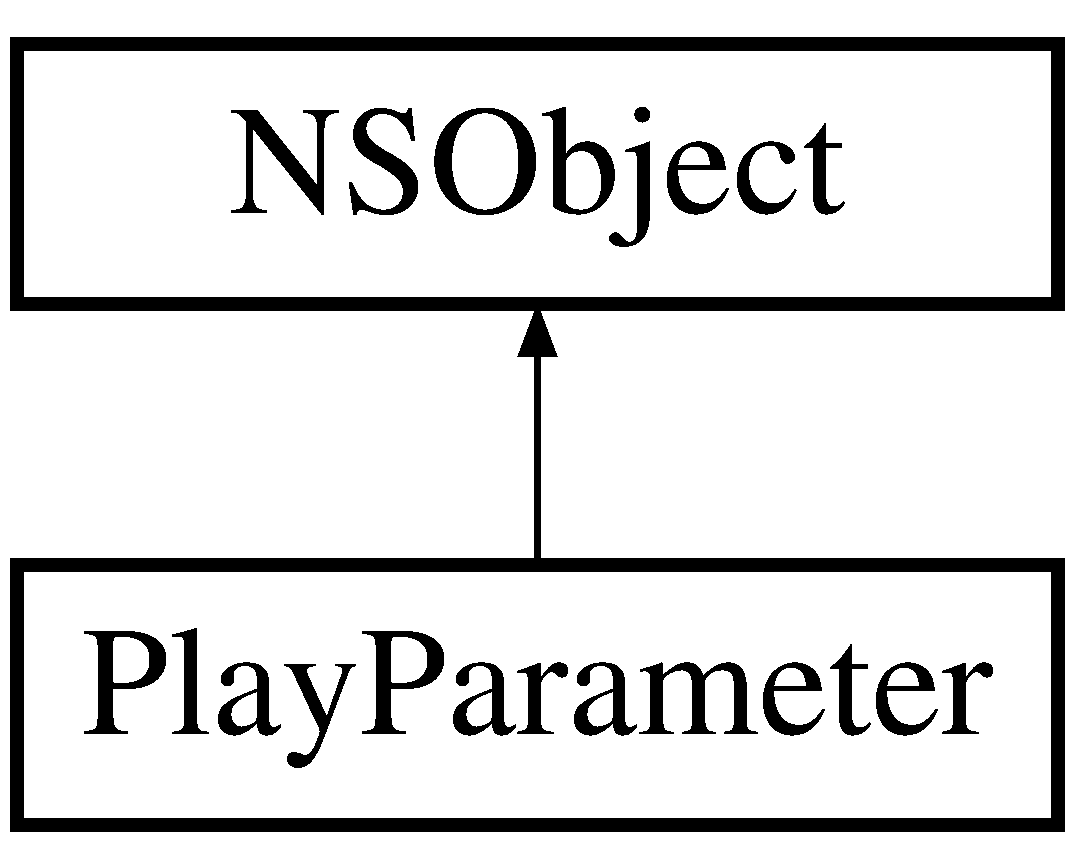
\includegraphics[height=2.000000cm]{interface_play_parameter}
\end{center}
\end{figure}
\subsection*{属性}
\begin{DoxyCompactItemize}
\item 
\mbox{\Hypertarget{interface_play_parameter_ae119336c7ec7ba46094c99d8fed265c4}\label{interface_play_parameter_ae119336c7ec7ba46094c99d8fed265c4}} 
N\+S\+String $\ast$ \hyperlink{interface_play_parameter_ae119336c7ec7ba46094c99d8fed265c4}{user\+Id}
\begin{DoxyCompactList}\small\item\em 用户\+ID \end{DoxyCompactList}\item 
\mbox{\Hypertarget{interface_play_parameter_acf58a41e3841d43aff70a5e6654e5bf4}\label{interface_play_parameter_acf58a41e3841d43aff70a5e6654e5bf4}} 
N\+S\+String $\ast$ \hyperlink{interface_play_parameter_acf58a41e3841d43aff70a5e6654e5bf4}{room\+Id}
\begin{DoxyCompactList}\small\item\em 房间\+ID \end{DoxyCompactList}\item 
\mbox{\Hypertarget{interface_play_parameter_a18fe5c0b0ec79d88b3e1c4484aeb2fc5}\label{interface_play_parameter_a18fe5c0b0ec79d88b3e1c4484aeb2fc5}} 
N\+S\+String $\ast$ \hyperlink{interface_play_parameter_a18fe5c0b0ec79d88b3e1c4484aeb2fc5}{viewer\+Name}
\begin{DoxyCompactList}\small\item\em 用户名称 \end{DoxyCompactList}\item 
\mbox{\Hypertarget{interface_play_parameter_ad3a9235ef0b1b0c755cc863472e17466}\label{interface_play_parameter_ad3a9235ef0b1b0c755cc863472e17466}} 
N\+S\+String $\ast$ \hyperlink{interface_play_parameter_ad3a9235ef0b1b0c755cc863472e17466}{token}
\begin{DoxyCompactList}\small\item\em 房间密码 \end{DoxyCompactList}\item 
\mbox{\Hypertarget{interface_play_parameter_a6ecb5ac7deee71e227f695a8a6aecc69}\label{interface_play_parameter_a6ecb5ac7deee71e227f695a8a6aecc69}} 
N\+S\+String $\ast$ \hyperlink{interface_play_parameter_a6ecb5ac7deee71e227f695a8a6aecc69}{live\+Id}
\begin{DoxyCompactList}\small\item\em 直播\+I\+D,回放时才用到 \end{DoxyCompactList}\item 
\mbox{\Hypertarget{interface_play_parameter_ac9b41020032b3931a22a01a8e5d80505}\label{interface_play_parameter_ac9b41020032b3931a22a01a8e5d80505}} 
N\+S\+String $\ast$ \hyperlink{interface_play_parameter_ac9b41020032b3931a22a01a8e5d80505}{record\+Id}
\begin{DoxyCompactList}\small\item\em 回放\+ID \end{DoxyCompactList}\item 
\mbox{\Hypertarget{interface_play_parameter_aa7bd8e47d7fb2fe8392fb93084cdcb40}\label{interface_play_parameter_aa7bd8e47d7fb2fe8392fb93084cdcb40}} 
N\+S\+String $\ast$ \hyperlink{interface_play_parameter_aa7bd8e47d7fb2fe8392fb93084cdcb40}{viewer\+Customua}
\begin{DoxyCompactList}\small\item\em 用户自定义参数,需和后台协商,没有定制传"" \end{DoxyCompactList}\item 
\mbox{\Hypertarget{interface_play_parameter_a47eb893bb06f765300978d0904aa8af0}\label{interface_play_parameter_a47eb893bb06f765300978d0904aa8af0}} 
N\+S\+String $\ast$ \hyperlink{interface_play_parameter_a47eb893bb06f765300978d0904aa8af0}{destination}
\begin{DoxyCompactList}\small\item\em 下载文件解压到的目录路径(离线下载相关) \end{DoxyCompactList}\item 
\mbox{\Hypertarget{interface_play_parameter_adfbc2b95a74fbbc79ed6dd387bdd0f36}\label{interface_play_parameter_adfbc2b95a74fbbc79ed6dd387bdd0f36}} 
U\+I\+View $\ast$ \hyperlink{interface_play_parameter_adfbc2b95a74fbbc79ed6dd387bdd0f36}{doc\+Parent}
\begin{DoxyCompactList}\small\item\em 文档父类窗口 \end{DoxyCompactList}\item 
\mbox{\Hypertarget{interface_play_parameter_ad36ae1eaafff8c3be9483521f18052c0}\label{interface_play_parameter_ad36ae1eaafff8c3be9483521f18052c0}} 
C\+G\+Rect \hyperlink{interface_play_parameter_ad36ae1eaafff8c3be9483521f18052c0}{doc\+Frame}
\begin{DoxyCompactList}\small\item\em 文档区域 \end{DoxyCompactList}\item 
\mbox{\Hypertarget{interface_play_parameter_a063b2a3b60adced28f74d6890d32d7af}\label{interface_play_parameter_a063b2a3b60adced28f74d6890d32d7af}} 
U\+I\+View $\ast$ \hyperlink{interface_play_parameter_a063b2a3b60adced28f74d6890d32d7af}{player\+Parent}
\begin{DoxyCompactList}\small\item\em 视频父类窗口 \end{DoxyCompactList}\item 
\mbox{\Hypertarget{interface_play_parameter_a3f824515b9c9cdcb05f2863423bd284b}\label{interface_play_parameter_a3f824515b9c9cdcb05f2863423bd284b}} 
C\+G\+Rect \hyperlink{interface_play_parameter_a3f824515b9c9cdcb05f2863423bd284b}{player\+Frame}
\begin{DoxyCompactList}\small\item\em 视频区域 \end{DoxyCompactList}\item 
\mbox{\Hypertarget{interface_play_parameter_ad58a58a2ca6913a15bdf5a80d5123d99}\label{interface_play_parameter_ad58a58a2ca6913a15bdf5a80d5123d99}} 
B\+O\+OL \hyperlink{interface_play_parameter_ad58a58a2ca6913a15bdf5a80d5123d99}{security}
\begin{DoxyCompactList}\small\item\em 是否使用https,静态库暂时只能使用http协议 \end{DoxyCompactList}\item 
\mbox{\Hypertarget{interface_play_parameter_a0a96b9ef62e69167ca1fb8b405e45119}\label{interface_play_parameter_a0a96b9ef62e69167ca1fb8b405e45119}} 
N\+S\+Integer \hyperlink{interface_play_parameter_a0a96b9ef62e69167ca1fb8b405e45119}{scaling\+Mode}
\begin{DoxyCompactList}\small\item\em 屏幕适配方式 0\+:I\+J\+K\+M\+P\+Movie\+Scaling\+Mode\+None 1\+:I\+J\+K\+M\+P\+Movie\+Scaling\+Mode\+Aspect\+Fit 2\+:I\+J\+K\+M\+P\+Movie\+Scaling\+Mode\+Aspect\+Fill 3\+:I\+J\+K\+M\+P\+Movie\+Scaling\+Mode\+Fill \end{DoxyCompactList}\item 
\mbox{\Hypertarget{interface_play_parameter_a0fc1c1924c6f27620ebc316cff688e54}\label{interface_play_parameter_a0fc1c1924c6f27620ebc316cff688e54}} 
U\+I\+Color $\ast$ \hyperlink{interface_play_parameter_a0fc1c1924c6f27620ebc316cff688e54}{default\+Color}
\begin{DoxyCompactList}\small\item\em ppt默认底色,不写默认为白色 \end{DoxyCompactList}\item 
\mbox{\Hypertarget{interface_play_parameter_a1044bc3b8162768a634f63d11689c6f9}\label{interface_play_parameter_a1044bc3b8162768a634f63d11689c6f9}} 
B\+O\+OL \hyperlink{interface_play_parameter_a1044bc3b8162768a634f63d11689c6f9}{pause\+In\+Back\+Ground}
\begin{DoxyCompactList}\small\item\em 后台是否继续播放,注意:如果开启后台播放需要打开 xcode-\/$>$Capabilities-\/$>$Background Modes-\/$>$on-\/$>$Audio,Air\+Play,and Picture in Picture \end{DoxyCompactList}\item 
N\+S\+Integer \hyperlink{interface_play_parameter_a515289628340de9b9e482191a48393e5}{P\+P\+T\+Scaling\+Mode}
\begin{DoxyCompactList}\small\item\em P\+P\+T适配模式分为三种, 1. \end{DoxyCompactList}\end{DoxyCompactItemize}


\subsection{属性说明}
\mbox{\Hypertarget{interface_play_parameter_a515289628340de9b9e482191a48393e5}\label{interface_play_parameter_a515289628340de9b9e482191a48393e5}} 
\index{Play\+Parameter@{Play\+Parameter}!P\+P\+T\+Scaling\+Mode@{P\+P\+T\+Scaling\+Mode}}
\index{P\+P\+T\+Scaling\+Mode@{P\+P\+T\+Scaling\+Mode}!Play\+Parameter@{Play\+Parameter}}
\subsubsection{\texorpdfstring{P\+P\+T\+Scaling\+Mode}{PPTScalingMode}}
{\footnotesize\ttfamily -\/ (N\+S\+Integer) P\+P\+T\+Scaling\+Mode\hspace{0.3cm}{\ttfamily [read]}, {\ttfamily [write]}, {\ttfamily [nonatomic]}, {\ttfamily [assign]}}



P\+P\+T适配模式分为三种, 1. 

一种是全部填充屏幕,可拉伸变形, 2.第二种是等比缩放,横向或竖向贴住边缘,另一方向可以留黑边, 3.第三种是等比缩放,横向或竖向贴住边缘,另一方向出边界,裁剪\+P\+P\+T,不可以留黑边 

该类的文档由以下文件生成\+:\begin{DoxyCompactItemize}
\item 
Play\+Parameter.\+h\end{DoxyCompactItemize}

\hypertarget{interface_request_data}{}\section{Request\+Data类 参考}
\label{interface_request_data}\index{Request\+Data@{Request\+Data}}
类 Request\+Data 继承关系图\+:\begin{figure}[H]
\begin{center}
\leavevmode
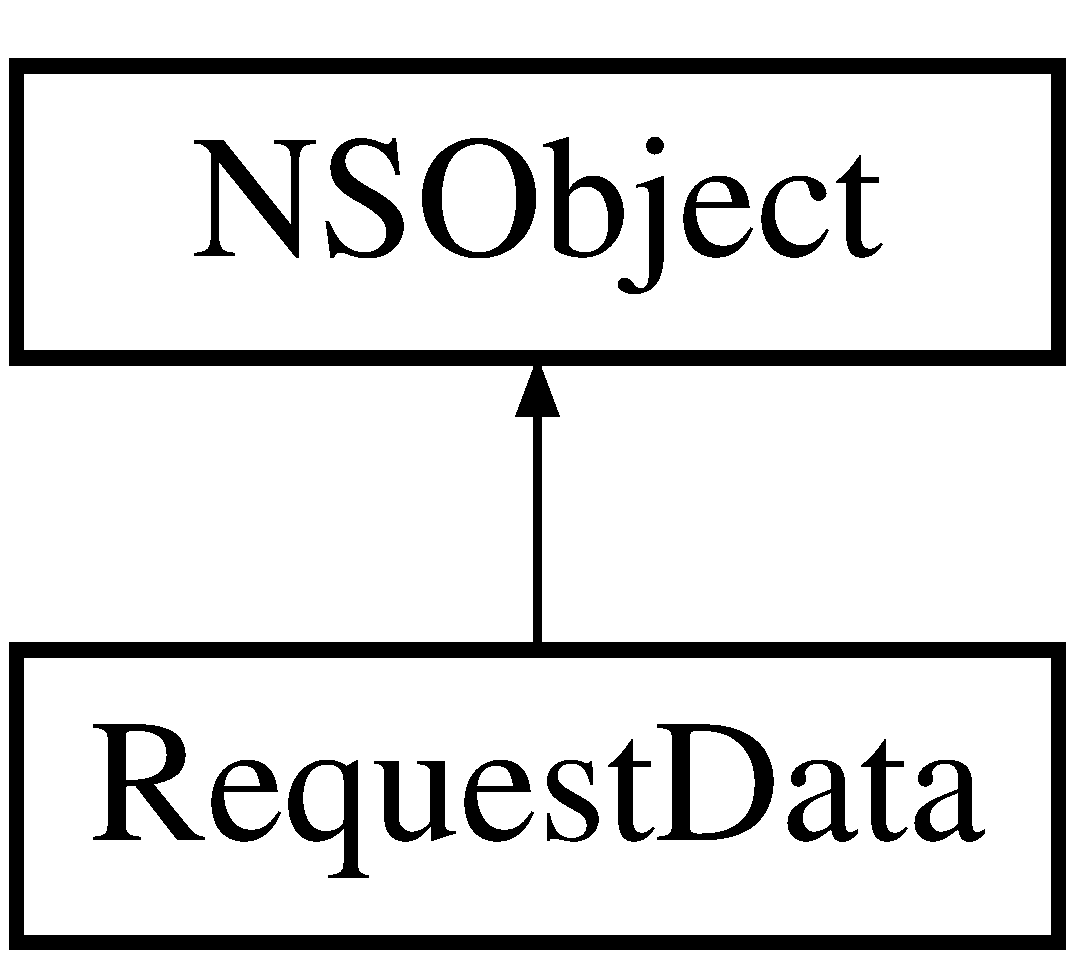
\includegraphics[height=2.000000cm]{interface_request_data}
\end{center}
\end{figure}
\subsection*{构造函数}
\begin{DoxyCompactItemize}
\item 
(id) -\/ \hyperlink{interface_request_data_aca8fabcea46e00a3e5a918f0668254f9}{init\+Login\+With\+Parameter\+:}
\begin{DoxyCompactList}\small\item\em 登录房间 \end{DoxyCompactList}\item 
(id) -\/ \hyperlink{interface_request_data_a67af7937b840135d7240c35aa5a5f78a}{init\+With\+Parameter\+:}
\begin{DoxyCompactList}\small\item\em 进入房间,并请求画图聊天数据并播放视频(可以不登陆,直接从此接口进入直播间) \end{DoxyCompactList}\item 
(void) -\/ \hyperlink{interface_request_data_a2e886316ef2970f8d97020221fe80c56}{question\+:}
\begin{DoxyCompactList}\small\item\em 提问 \end{DoxyCompactList}\item 
(void) -\/ \hyperlink{interface_request_data_ae859b4435402fd2c676f43fa3ba1fcf1}{chat\+Message\+:}
\begin{DoxyCompactList}\small\item\em 发送公聊信息 \end{DoxyCompactList}\item 
\mbox{\Hypertarget{interface_request_data_a2b64c1bf11fd8476f06f663f1df9fefa}\label{interface_request_data_a2b64c1bf11fd8476f06f663f1df9fefa}} 
(void) -\/ \hyperlink{interface_request_data_a2b64c1bf11fd8476f06f663f1df9fefa}{private\+Chat\+With\+Touserid\+:msg\+:}
\begin{DoxyCompactList}\small\item\em 发送私聊信息 \end{DoxyCompactList}\item 
\mbox{\Hypertarget{interface_request_data_a7af614d3cf16583da1df36ab5c4b45b9}\label{interface_request_data_a7af614d3cf16583da1df36ab5c4b45b9}} 
(void) -\/ \hyperlink{interface_request_data_a7af614d3cf16583da1df36ab5c4b45b9}{request\+Cancel}
\begin{DoxyCompactList}\small\item\em 销毁文档和视频,清除视频和文档的时候需要调用,推出播放页面的时候也需要调用 \end{DoxyCompactList}\item 
\mbox{\Hypertarget{interface_request_data_a626619664a5b87e0283f2c4f4b6231cb}\label{interface_request_data_a626619664a5b87e0283f2c4f4b6231cb}} 
(void) -\/ \hyperlink{interface_request_data_a626619664a5b87e0283f2c4f4b6231cb}{room\+User\+Count}
\begin{DoxyCompactList}\small\item\em 获取在线房间人数,当登录成功后即可调用此接口,登录不成功或者退出登录后就不可以调用了,如果要求实时性比较强的话,可以写一个定时器,不断调用此接口,几秒钟发一次就可以,然后在代理回调函数中,处理返回的数据 \end{DoxyCompactList}\item 
\mbox{\Hypertarget{interface_request_data_a2557f6728b0797aa4021a48ea0b21252}\label{interface_request_data_a2557f6728b0797aa4021a48ea0b21252}} 
(C\+G\+Float) -\/ \hyperlink{interface_request_data_a2557f6728b0797aa4021a48ea0b21252}{get\+Doc\+Aspect\+Ratio}
\begin{DoxyCompactList}\small\item\em 获取文档区域内白板或者文档本身的宽高比,返回值即为宽高比,做屏幕适配用 \end{DoxyCompactList}\item 
\mbox{\Hypertarget{interface_request_data_a6bd441ac80191c90f9283709da9895c1}\label{interface_request_data_a6bd441ac80191c90f9283709da9895c1}} 
(void) -\/ \hyperlink{interface_request_data_a6bd441ac80191c90f9283709da9895c1}{change\+Doc\+Frame\+:}
\begin{DoxyCompactList}\small\item\em 改变文档区域大小,主要用在文档生成后改变文档窗口的frame \end{DoxyCompactList}\item 
\mbox{\Hypertarget{interface_request_data_a7d242ff8ab02b40741f8e1a75d785ec7}\label{interface_request_data_a7d242ff8ab02b40741f8e1a75d785ec7}} 
(void) -\/ \hyperlink{interface_request_data_a7d242ff8ab02b40741f8e1a75d785ec7}{change\+Player\+Frame\+:}
\begin{DoxyCompactList}\small\item\em 改变播放器frame \end{DoxyCompactList}\item 
\mbox{\Hypertarget{interface_request_data_aab62970b8d882746572a97f32992a5ae}\label{interface_request_data_aab62970b8d882746572a97f32992a5ae}} 
(void) -\/ \hyperlink{interface_request_data_aab62970b8d882746572a97f32992a5ae}{change\+Player\+Parent\+:}
\begin{DoxyCompactList}\small\item\em 改变播放器父窗口 \end{DoxyCompactList}\item 
\mbox{\Hypertarget{interface_request_data_a37719945b113eff0941f5a1212ae9216}\label{interface_request_data_a37719945b113eff0941f5a1212ae9216}} 
(void) -\/ \hyperlink{interface_request_data_a37719945b113eff0941f5a1212ae9216}{change\+Doc\+Parent\+:}
\begin{DoxyCompactList}\small\item\em 改变文档父窗口 \end{DoxyCompactList}\item 
\mbox{\Hypertarget{interface_request_data_afa31c9712b6356fcaee24267d43863e3}\label{interface_request_data_afa31c9712b6356fcaee24267d43863e3}} 
(void) -\/ \hyperlink{interface_request_data_afa31c9712b6356fcaee24267d43863e3}{pause\+Player}
\begin{DoxyCompactList}\small\item\em 播放器暂停 \end{DoxyCompactList}\item 
\mbox{\Hypertarget{interface_request_data_a26f668c79f901d70090f4d25f925e62f}\label{interface_request_data_a26f668c79f901d70090f4d25f925e62f}} 
(void) -\/ \hyperlink{interface_request_data_a26f668c79f901d70090f4d25f925e62f}{start\+Player}
\begin{DoxyCompactList}\small\item\em 播放器播放 \end{DoxyCompactList}\item 
\mbox{\Hypertarget{interface_request_data_a5fa79092e740b86134c113e8f1beea22}\label{interface_request_data_a5fa79092e740b86134c113e8f1beea22}} 
(void) -\/ \hyperlink{interface_request_data_a5fa79092e740b86134c113e8f1beea22}{shutdown\+Player}
\begin{DoxyCompactList}\small\item\em 播放器关闭并移除 \end{DoxyCompactList}\item 
\mbox{\Hypertarget{interface_request_data_ae509e7097cd3ddfad8f0b81dd51eff33}\label{interface_request_data_ae509e7097cd3ddfad8f0b81dd51eff33}} 
(void) -\/ \hyperlink{interface_request_data_ae509e7097cd3ddfad8f0b81dd51eff33}{stop\+Player}
\begin{DoxyCompactList}\small\item\em 播放器停止 \end{DoxyCompactList}\item 
\mbox{\Hypertarget{interface_request_data_a614c0a62c3d2bb301473c91c3a5a2991}\label{interface_request_data_a614c0a62c3d2bb301473c91c3a5a2991}} 
(void) -\/ \hyperlink{interface_request_data_a614c0a62c3d2bb301473c91c3a5a2991}{switch\+To\+Play\+Url\+With\+Fir\+Index\+:key\+:}
\begin{DoxyCompactList}\small\item\em 切换播放线路 fir\+Index表示第几个源 key表示该源对应的描述信息 \end{DoxyCompactList}\item 
\mbox{\Hypertarget{interface_request_data_acbe1b2db40350e4f5fb4e714e3303ccd}\label{interface_request_data_acbe1b2db40350e4f5fb4e714e3303ccd}} 
(void) -\/ \hyperlink{interface_request_data_acbe1b2db40350e4f5fb4e714e3303ccd}{reload\+Video\+:}
\begin{DoxyCompactList}\small\item\em 重新加载视频,参数force表示是否强制重新加载视频, 一般重新加载视频的时间间隔应该超过3秒,如果强制重新加载视频,时间间隔可以在3\+S之内 \end{DoxyCompactList}\item 
\mbox{\Hypertarget{interface_request_data_a0111d63c6e3a42932722a36a673c8645}\label{interface_request_data_a0111d63c6e3a42932722a36a673c8645}} 
(void) -\/ \hyperlink{interface_request_data_a0111d63c6e3a42932722a36a673c8645}{answer\+\_\+rollcall}
\begin{DoxyCompactList}\small\item\em 签到 \end{DoxyCompactList}\item 
\mbox{\Hypertarget{interface_request_data_a78dbd275a2d087ae7528ba0550891623}\label{interface_request_data_a78dbd275a2d087ae7528ba0550891623}} 
(void) -\/ \hyperlink{interface_request_data_a78dbd275a2d087ae7528ba0550891623}{reply\+\_\+vote\+\_\+single\+:}
\begin{DoxyCompactList}\small\item\em 答单选题 \end{DoxyCompactList}\item 
\mbox{\Hypertarget{interface_request_data_afbac7a33f1e2f07f1e5e53bbfc9e829d}\label{interface_request_data_afbac7a33f1e2f07f1e5e53bbfc9e829d}} 
(void) -\/ \hyperlink{interface_request_data_afbac7a33f1e2f07f1e5e53bbfc9e829d}{reply\+\_\+vote\+\_\+multiple\+:}
\begin{DoxyCompactList}\small\item\em 答多选题 \end{DoxyCompactList}\item 
\mbox{\Hypertarget{interface_request_data_acbef681a6e74e8eb85c9f4c3725eac49}\label{interface_request_data_acbef681a6e74e8eb85c9f4c3725eac49}} 
(B\+O\+OL) -\/ \hyperlink{interface_request_data_acbef681a6e74e8eb85c9f4c3725eac49}{is\+Playing}
\begin{DoxyCompactList}\small\item\em 播放器是否播放 \end{DoxyCompactList}\item 
\mbox{\Hypertarget{interface_request_data_a8fbbb99919a9c8b04d62d131d4e1f013}\label{interface_request_data_a8fbbb99919a9c8b04d62d131d4e1f013}} 
(void) -\/ \hyperlink{interface_request_data_a8fbbb99919a9c8b04d62d131d4e1f013}{setpause\+In\+Back\+Ground\+:}
\begin{DoxyCompactList}\small\item\em 设置后台是否可播放 \end{DoxyCompactList}\item 
\mbox{\Hypertarget{interface_request_data_a38c258894bd7f0afb2820a0d7bd50658}\label{interface_request_data_a38c258894bd7f0afb2820a0d7bd50658}} 
(void) -\/ \hyperlink{interface_request_data_a38c258894bd7f0afb2820a0d7bd50658}{commit\+Questionnaire\+:}
\begin{DoxyCompactList}\small\item\em 提交问卷结果 \end{DoxyCompactList}\item 
\mbox{\Hypertarget{interface_request_data_a398f1c6f00717a09ce27aa994aba4ec8}\label{interface_request_data_a398f1c6f00717a09ce27aa994aba4ec8}} 
(void) -\/ \hyperlink{interface_request_data_a398f1c6f00717a09ce27aa994aba4ec8}{get\+Publishing\+Questionnaire}
\begin{DoxyCompactList}\small\item\em 主动请求问卷 \end{DoxyCompactList}\item 
\mbox{\Hypertarget{interface_request_data_ad41b048ed7dd6dafd40543e5e8cb8bd0}\label{interface_request_data_ad41b048ed7dd6dafd40543e5e8cb8bd0}} 
(void) -\/ \hyperlink{interface_request_data_ad41b048ed7dd6dafd40543e5e8cb8bd0}{save\+User\+Info\+:remote\+View\+:}
\begin{DoxyCompactList}\small\item\em 当收到-\/ (void)accept\+Speak\+:(\+N\+S\+Dictionary $\ast$)dict;回调方法后,调用此方法 dict 正是-\/ (void)accept\+Speak\+:(\+N\+S\+Dictionary $\ast$)dict;接收到的的参数 remote\+View 是远程连麦页面的view,需要自己设置并发给\+S\+D\+K,\+S\+D\+K将要在这个view上进行远程画面渲染 \end{DoxyCompactList}\item 
\mbox{\Hypertarget{interface_request_data_aebd00f94f73a4a0e8f844a70587dc862}\label{interface_request_data_aebd00f94f73a4a0e8f844a70587dc862}} 
(void) -\/ \hyperlink{interface_request_data_aebd00f94f73a4a0e8f844a70587dc862}{dis\+Connect\+Speak}
\begin{DoxyCompactList}\small\item\em 观看端主动断开连麦时候需要调用的接口 \end{DoxyCompactList}\item 
\mbox{\Hypertarget{interface_request_data_a09409a59e7cafc7573f2692d5d951851}\label{interface_request_data_a09409a59e7cafc7573f2692d5d951851}} 
(void) -\/ \hyperlink{interface_request_data_a09409a59e7cafc7573f2692d5d951851}{request\+A\+V\+Message\+With\+Local\+View\+:is\+Audio\+Video\+:}
\begin{DoxyCompactList}\small\item\em 当观看端主动申请连麦时,需要调用这个接口,并把本地连麦预览窗口传给\+S\+D\+K,\+S\+D\+K会在这个view上 进行远程画面渲染 param local\+View\+:本地预览窗口,传入本地view,连麦准备时间将会自动绘制预览画面在此view上 param is\+Audio\+Video\+:是否是音视频连麦,不是音视频即是纯音频连麦(Y\+E\+S表示音视频连麦,\+N\+O表示音频连麦) \end{DoxyCompactList}\item 
\mbox{\Hypertarget{interface_request_data_a8172beb9c4d7a8fc9b19610c671f827f}\label{interface_request_data_a8172beb9c4d7a8fc9b19610c671f827f}} 
(void) -\/ \hyperlink{interface_request_data_a8172beb9c4d7a8fc9b19610c671f827f}{set\+Local\+Video\+Frame\+A\+:}
\begin{DoxyCompactList}\small\item\em 设置本地预览窗口的大小,连麦成功后调用才生效,连麦不成功调用不生效 \end{DoxyCompactList}\item 
\mbox{\Hypertarget{interface_request_data_a4d582d2ae5f8d0db746bd6652934e9dd}\label{interface_request_data_a4d582d2ae5f8d0db746bd6652934e9dd}} 
(void) -\/ \hyperlink{interface_request_data_a4d582d2ae5f8d0db746bd6652934e9dd}{set\+Remote\+Video\+Frame\+A\+:}
\begin{DoxyCompactList}\small\item\em 设置远程连麦窗口的大小,连麦成功后调用才生效,连麦不成功调用不生效 \end{DoxyCompactList}\item 
\mbox{\Hypertarget{interface_request_data_a73cdccb2fbc387504c9de85443b047a6}\label{interface_request_data_a73cdccb2fbc387504c9de85443b047a6}} 
(void) -\/ \hyperlink{interface_request_data_a73cdccb2fbc387504c9de85443b047a6}{goto\+Connect\+Web\+R\+TC}
\begin{DoxyCompactList}\small\item\em 将要连接\+Web\+R\+TC \end{DoxyCompactList}\end{DoxyCompactItemize}
\subsection*{属性}
\begin{DoxyCompactItemize}
\item 
\mbox{\Hypertarget{interface_request_data_a5c7c46d4aececcd6cae8cdd6caf28f52}\label{interface_request_data_a5c7c46d4aececcd6cae8cdd6caf28f52}} 
id$<$ Request\+Data\+Delegate $>$ \hyperlink{interface_request_data_a5c7c46d4aececcd6cae8cdd6caf28f52}{delegate}
\begin{DoxyCompactList}\small\item\em 代理 \end{DoxyCompactList}\item 
\mbox{\Hypertarget{interface_request_data_a6d47af84efb44378a2bf9a87830a86be}\label{interface_request_data_a6d47af84efb44378a2bf9a87830a86be}} 
id$<$ I\+J\+K\+Media\+Playback $>$ \hyperlink{interface_request_data_a6d47af84efb44378a2bf9a87830a86be}{ijk\+Player}
\begin{DoxyCompactList}\small\item\em 播放器 \end{DoxyCompactList}\end{DoxyCompactItemize}


\subsection{函数文档}
\mbox{\Hypertarget{interface_request_data_ae859b4435402fd2c676f43fa3ba1fcf1}\label{interface_request_data_ae859b4435402fd2c676f43fa3ba1fcf1}} 
\index{Request\+Data@{Request\+Data}!chat\+Message\+:@{chat\+Message\+:}}
\index{chat\+Message\+:@{chat\+Message\+:}!Request\+Data@{Request\+Data}}
\subsubsection{\texorpdfstring{chat\+Message\+:()}{chatMessage:()}}
{\footnotesize\ttfamily -\/ (void) chat\+Message\+: \begin{DoxyParamCaption}\item[{(N\+S\+String $\ast$)}]{message }\end{DoxyParamCaption}}



发送公聊信息 


\begin{DoxyParams}{参数}
{\em message} & 发送的消息内容 \\
\hline
\end{DoxyParams}
\mbox{\Hypertarget{interface_request_data_aca8fabcea46e00a3e5a918f0668254f9}\label{interface_request_data_aca8fabcea46e00a3e5a918f0668254f9}} 
\index{Request\+Data@{Request\+Data}!init\+Login\+With\+Parameter\+:@{init\+Login\+With\+Parameter\+:}}
\index{init\+Login\+With\+Parameter\+:@{init\+Login\+With\+Parameter\+:}!Request\+Data@{Request\+Data}}
\subsubsection{\texorpdfstring{init\+Login\+With\+Parameter\+:()}{initLoginWithParameter:()}}
{\footnotesize\ttfamily -\/ (id) init\+Login\+With\+Parameter\+: \begin{DoxyParamCaption}\item[{(\hyperlink{interface_play_parameter}{Play\+Parameter} $\ast$)}]{parameter }\end{DoxyParamCaption}}



登录房间 


\begin{DoxyParams}{参数}
{\em parameter} & 配置参数信息 必填参数 user\+Id; 必填参数 room\+Id; 必填参数 viewer\+Name; 必填参数 token; 必填参数 security; (选填参数) viewercustomua; \\
\hline
\end{DoxyParams}
\mbox{\Hypertarget{interface_request_data_a67af7937b840135d7240c35aa5a5f78a}\label{interface_request_data_a67af7937b840135d7240c35aa5a5f78a}} 
\index{Request\+Data@{Request\+Data}!init\+With\+Parameter\+:@{init\+With\+Parameter\+:}}
\index{init\+With\+Parameter\+:@{init\+With\+Parameter\+:}!Request\+Data@{Request\+Data}}
\subsubsection{\texorpdfstring{init\+With\+Parameter\+:()}{initWithParameter:()}}
{\footnotesize\ttfamily -\/ (id) init\+With\+Parameter\+: \begin{DoxyParamCaption}\item[{(\hyperlink{interface_play_parameter}{Play\+Parameter} $\ast$)}]{parameter }\end{DoxyParamCaption}}



进入房间,并请求画图聊天数据并播放视频(可以不登陆,直接从此接口进入直播间) 


\begin{DoxyParams}{参数}
{\em parameter} & 配置参数信息 必填参数 user\+Id; 必填参数 room\+Id; 必填参数 viewer\+Name; 必填参数 token; 必填参数 doc\+Parent; 必填参数 doc\+Frame; 必填参数 player\+Parent; 必填参数 player\+Frame; 必填参数 scaling\+Mode; 必填参数 security; 必填参数 default\+Color; 必填参数 scaling\+Mode; 必填参数 P\+P\+T\+Scaling\+Mode; 必填参数 pause\+In\+Back\+Ground; (选填参数) viewercustomua; \\
\hline
\end{DoxyParams}
\mbox{\Hypertarget{interface_request_data_a2e886316ef2970f8d97020221fe80c56}\label{interface_request_data_a2e886316ef2970f8d97020221fe80c56}} 
\index{Request\+Data@{Request\+Data}!question\+:@{question\+:}}
\index{question\+:@{question\+:}!Request\+Data@{Request\+Data}}
\subsubsection{\texorpdfstring{question\+:()}{question:()}}
{\footnotesize\ttfamily -\/ (void) question\+: \begin{DoxyParamCaption}\item[{(N\+S\+String $\ast$)}]{message }\end{DoxyParamCaption}}



提问 


\begin{DoxyParams}{参数}
{\em message} & 提问内容 \\
\hline
\end{DoxyParams}


该类的文档由以下文件生成\+:\begin{DoxyCompactItemize}
\item 
Request\+Data.\+h\end{DoxyCompactItemize}

\hypertarget{protocol_request_data_delegate_01-p}{}\section{$<$Request\+Data\+Delegate $>$协议 参考}
\label{protocol_request_data_delegate_01-p}\index{$<$\+Request\+Data\+Delegate $>$@{$<$\+Request\+Data\+Delegate $>$}}
类 $<$Request\+Data\+Delegate $>$ 继承关系图\+:\begin{figure}[H]
\begin{center}
\leavevmode
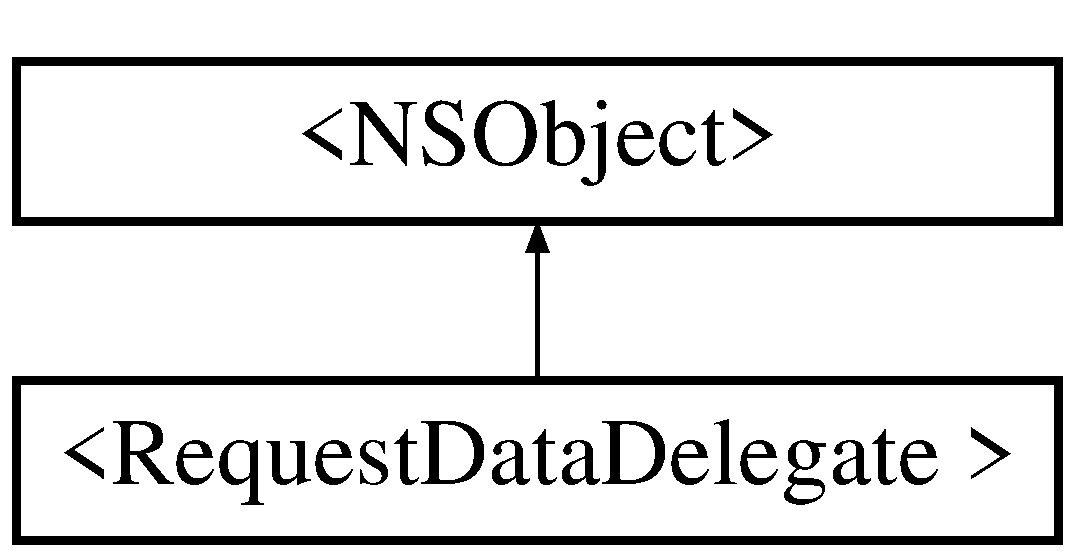
\includegraphics[height=2.000000cm]{protocol_request_data_delegate_01-p}
\end{center}
\end{figure}
\subsection*{构造函数}
\begin{DoxyCompactItemize}
\item 
\mbox{\Hypertarget{protocol_request_data_delegate_01-p_abf987c7b327a9df5fb1d6eff506832fd}\label{protocol_request_data_delegate_01-p_abf987c7b327a9df5fb1d6eff506832fd}} 
(void) -\/ \hyperlink{protocol_request_data_delegate_01-p_abf987c7b327a9df5fb1d6eff506832fd}{request\+Succeed}
\begin{DoxyCompactList}\small\item\em 请求播放地址成功 \end{DoxyCompactList}\item 
\mbox{\Hypertarget{protocol_request_data_delegate_01-p_a0df0d78d55862f66b70dca75264bbc12}\label{protocol_request_data_delegate_01-p_a0df0d78d55862f66b70dca75264bbc12}} 
(void) -\/ \hyperlink{protocol_request_data_delegate_01-p_a0df0d78d55862f66b70dca75264bbc12}{request\+Failed\+:reason\+:}
\begin{DoxyCompactList}\small\item\em 请求播放地址失败 \end{DoxyCompactList}\item 
\mbox{\Hypertarget{protocol_request_data_delegate_01-p_a7341816ad8c4bbda620c7783d8a3568d}\label{protocol_request_data_delegate_01-p_a7341816ad8c4bbda620c7783d8a3568d}} 
(void) -\/ \hyperlink{protocol_request_data_delegate_01-p_a7341816ad8c4bbda620c7783d8a3568d}{on\+Question\+Dic\+:}
\begin{DoxyCompactList}\small\item\em 收到提问,用户观看时和主讲的互动问答信息 \end{DoxyCompactList}\item 
\mbox{\Hypertarget{protocol_request_data_delegate_01-p_ae5a9d7514c6ad8c448dfb3e332bc5cf8}\label{protocol_request_data_delegate_01-p_ae5a9d7514c6ad8c448dfb3e332bc5cf8}} 
(void) -\/ \hyperlink{protocol_request_data_delegate_01-p_ae5a9d7514c6ad8c448dfb3e332bc5cf8}{on\+Answer\+Dic\+:}
\begin{DoxyCompactList}\small\item\em 收到回答,用户观看时和主讲的互动问答信息 \end{DoxyCompactList}\item 
\mbox{\Hypertarget{protocol_request_data_delegate_01-p_a5995fc6c05c04b1f0a16469d574a5cd5}\label{protocol_request_data_delegate_01-p_a5995fc6c05c04b1f0a16469d574a5cd5}} 
(void) -\/ \hyperlink{protocol_request_data_delegate_01-p_a5995fc6c05c04b1f0a16469d574a5cd5}{on\+Question\+Arr\+:on\+Answer\+Arr\+:}
\begin{DoxyCompactList}\small\item\em 收到提问\&回答,在用户登录之前,主讲和其他用户的历史互动问答信息 \end{DoxyCompactList}\item 
\mbox{\Hypertarget{protocol_request_data_delegate_01-p_a1c0314c63eb388f7a3bd177a5dcb797c}\label{protocol_request_data_delegate_01-p_a1c0314c63eb388f7a3bd177a5dcb797c}} 
(void) -\/ \hyperlink{protocol_request_data_delegate_01-p_a1c0314c63eb388f7a3bd177a5dcb797c}{on\+Chat\+Log\+:}
\begin{DoxyCompactList}\small\item\em 历史聊天数据 \end{DoxyCompactList}\item 
\mbox{\Hypertarget{protocol_request_data_delegate_01-p_aafe0d41665c810e8f42fa0482711ff10}\label{protocol_request_data_delegate_01-p_aafe0d41665c810e8f42fa0482711ff10}} 
(void) -\/ \hyperlink{protocol_request_data_delegate_01-p_aafe0d41665c810e8f42fa0482711ff10}{on\+Live\+Status\+Change\+Start}
\begin{DoxyCompactList}\small\item\em 主讲开始推流 \end{DoxyCompactList}\item 
\mbox{\Hypertarget{protocol_request_data_delegate_01-p_a3f81e1f0908d02f763bd3de8648de94f}\label{protocol_request_data_delegate_01-p_a3f81e1f0908d02f763bd3de8648de94f}} 
(void) -\/ \hyperlink{protocol_request_data_delegate_01-p_a3f81e1f0908d02f763bd3de8648de94f}{on\+Live\+Status\+Change\+End\+:}
\begin{DoxyCompactList}\small\item\em 停止直播,end\+Normal表示是否异常停止推流,这个参数对观看端影响不大 \end{DoxyCompactList}\item 
\mbox{\Hypertarget{protocol_request_data_delegate_01-p_a42345c7ea7ded09062d66ace74419ed2}\label{protocol_request_data_delegate_01-p_a42345c7ea7ded09062d66ace74419ed2}} 
(void) -\/ \hyperlink{protocol_request_data_delegate_01-p_a42345c7ea7ded09062d66ace74419ed2}{on\+Public\+Chat\+Message\+:}
\begin{DoxyCompactList}\small\item\em 收到公聊消息 \end{DoxyCompactList}\item 
\mbox{\Hypertarget{protocol_request_data_delegate_01-p_a5408d30b923a72a0f667fc7b074d4792}\label{protocol_request_data_delegate_01-p_a5408d30b923a72a0f667fc7b074d4792}} 
(void) -\/ \hyperlink{protocol_request_data_delegate_01-p_a5408d30b923a72a0f667fc7b074d4792}{On\+Private\+Chat\+:}
\begin{DoxyCompactList}\small\item\em 收到私聊信息 \end{DoxyCompactList}\item 
\mbox{\Hypertarget{protocol_request_data_delegate_01-p_a3f2560687b42d6a4eb2e3e531c42c3cc}\label{protocol_request_data_delegate_01-p_a3f2560687b42d6a4eb2e3e531c42c3cc}} 
(void) -\/ \hyperlink{protocol_request_data_delegate_01-p_a3f2560687b42d6a4eb2e3e531c42c3cc}{on\+Silence\+User\+Chat\+Message\+:}
\begin{DoxyCompactList}\small\item\em 收到自己的禁言消息,如果你被禁言了,你发出的消息只有你自己能看到,其他人看不到 \end{DoxyCompactList}\item 
\mbox{\Hypertarget{protocol_request_data_delegate_01-p_ac6835dc0e86081b1d6800da29653f39a}\label{protocol_request_data_delegate_01-p_ac6835dc0e86081b1d6800da29653f39a}} 
(void) -\/ \hyperlink{protocol_request_data_delegate_01-p_ac6835dc0e86081b1d6800da29653f39a}{on\+User\+Count\+:}
\begin{DoxyCompactList}\small\item\em 收到在线人数 \end{DoxyCompactList}\item 
\mbox{\Hypertarget{protocol_request_data_delegate_01-p_affce5046a6aad966caa3a1d46fd3eaf3}\label{protocol_request_data_delegate_01-p_affce5046a6aad966caa3a1d46fd3eaf3}} 
(void) -\/ \hyperlink{protocol_request_data_delegate_01-p_affce5046a6aad966caa3a1d46fd3eaf3}{information\+:}
\begin{DoxyCompactList}\small\item\em 当主讲全体禁言时,你再发消息,会出发此代理方法,information是禁言提示信息 \end{DoxyCompactList}\item 
\mbox{\Hypertarget{protocol_request_data_delegate_01-p_a65e153a53b88a4fceb9ef31f88034397}\label{protocol_request_data_delegate_01-p_a65e153a53b88a4fceb9ef31f88034397}} 
(void) -\/ \hyperlink{protocol_request_data_delegate_01-p_a65e153a53b88a4fceb9ef31f88034397}{set\+My\+Viewer\+Id\+:}
\begin{DoxyCompactList}\small\item\em 服务器端给自己设置的\+User\+Id \end{DoxyCompactList}\item 
\mbox{\Hypertarget{protocol_request_data_delegate_01-p_acaeb6327cf94945d0961ce485d63179d}\label{protocol_request_data_delegate_01-p_acaeb6327cf94945d0961ce485d63179d}} 
(void) -\/ \hyperlink{protocol_request_data_delegate_01-p_acaeb6327cf94945d0961ce485d63179d}{on\+Kick\+Out}
\begin{DoxyCompactList}\small\item\em 收到踢出消息,停止推流并退出播放(被主播踢出) \end{DoxyCompactList}\item 
\mbox{\Hypertarget{protocol_request_data_delegate_01-p_ac7e7129cc172dba4b35a4bf35a86ae16}\label{protocol_request_data_delegate_01-p_ac7e7129cc172dba4b35a4bf35a86ae16}} 
(void) -\/ \hyperlink{protocol_request_data_delegate_01-p_ac7e7129cc172dba4b35a4bf35a86ae16}{room\+Info\+:}
\begin{DoxyCompactList}\small\item\em 获取房间信息,主要是要获取直播间模版来类型,根据直播间模版类型来确定界面布局 房间简介:dic\mbox{[}"desc\char`\"{}\mbox{]};
房间名称:dic\mbox{[}@\char`\"{}name\char`\"{}\mbox{]};
房间模版类型:\mbox{[}dic\mbox{[}@\char`\"{}template\+Type"\mbox{]} integer\+Value\mbox{]}; 模版类型为1\+: 聊天互动: 无 直播文档: 无 直播问答: 无 模版类型为2\+: 聊天互动: 有 直播文档: 无 直播问答: 有 模版类型为3\+: 聊天互动: 有 直播文档: 无 直播问答: 无 模版类型为4\+: 聊天互动: 有 直播文档: 有 直播问答: 无 模版类型为5\+: 聊天互动: 有 直播文档: 有 直播问答: 有 模版类型为6\+: 聊天互动: 无 直播文档: 无 直播问答: 有 \end{DoxyCompactList}\item 
\mbox{\Hypertarget{protocol_request_data_delegate_01-p_ad968ef491836696e905e599e3a412ea4}\label{protocol_request_data_delegate_01-p_ad968ef491836696e905e599e3a412ea4}} 
(void) -\/ \hyperlink{protocol_request_data_delegate_01-p_ad968ef491836696e905e599e3a412ea4}{get\+Play\+Statue\+:}
\begin{DoxyCompactList}\small\item\em 收到播放直播状态 0直播 1未直播 \end{DoxyCompactList}\item 
\mbox{\Hypertarget{protocol_request_data_delegate_01-p_ac4d791a2d5293df912eb07d8b3073829}\label{protocol_request_data_delegate_01-p_ac4d791a2d5293df912eb07d8b3073829}} 
(void) -\/ \hyperlink{protocol_request_data_delegate_01-p_ac4d791a2d5293df912eb07d8b3073829}{get\+Doc\+Aspect\+Ratio\+Of\+Width\+:height\+:}
\begin{DoxyCompactList}\small\item\em 获取文档内白板或者文档本身的宽高,来进行屏幕适配用的 \end{DoxyCompactList}\item 
\mbox{\Hypertarget{protocol_request_data_delegate_01-p_af29017f1177c5a14957dc3453238a171}\label{protocol_request_data_delegate_01-p_af29017f1177c5a14957dc3453238a171}} 
(void) -\/ \hyperlink{protocol_request_data_delegate_01-p_af29017f1177c5a14957dc3453238a171}{login\+Succeed\+Play}
\begin{DoxyCompactList}\small\item\em 登录成功 \end{DoxyCompactList}\item 
\mbox{\Hypertarget{protocol_request_data_delegate_01-p_aa998619e251865f7794128131f6b9036}\label{protocol_request_data_delegate_01-p_aa998619e251865f7794128131f6b9036}} 
(void) -\/ \hyperlink{protocol_request_data_delegate_01-p_aa998619e251865f7794128131f6b9036}{login\+Failed\+:reason\+:}
\begin{DoxyCompactList}\small\item\em 登录失败 \end{DoxyCompactList}\item 
\mbox{\Hypertarget{protocol_request_data_delegate_01-p_af2d37b5ea9d76ea558e86611f76c5914}\label{protocol_request_data_delegate_01-p_af2d37b5ea9d76ea558e86611f76c5914}} 
(void) -\/ \hyperlink{protocol_request_data_delegate_01-p_af2d37b5ea9d76ea558e86611f76c5914}{fir\+Road\+:sec\+Road\+Key\+Array\+:}
\begin{DoxyCompactList}\small\item\em 切换源,fir\+Road\+Num表示一共有几个源,sec\+Road\+Key\+Array表示每 个源的描述数组,具体参见demo,fir\+Road\+Num是下拉列表有面的tableviewcell 的行数,sec\+Road\+Key\+Array是左面的tableviewcell的描述信息数组 \end{DoxyCompactList}\item 
\mbox{\Hypertarget{protocol_request_data_delegate_01-p_ab78c990f513cf34d1990fd5ca7232336}\label{protocol_request_data_delegate_01-p_ab78c990f513cf34d1990fd5ca7232336}} 
(void) -\/ \hyperlink{protocol_request_data_delegate_01-p_ab78c990f513cf34d1990fd5ca7232336}{custom\+Message\+:}
\begin{DoxyCompactList}\small\item\em 自定义消息 \end{DoxyCompactList}\item 
\mbox{\Hypertarget{protocol_request_data_delegate_01-p_a084dbfc940ff86d96629ef6497692cbb}\label{protocol_request_data_delegate_01-p_a084dbfc940ff86d96629ef6497692cbb}} 
(void) -\/ \hyperlink{protocol_request_data_delegate_01-p_a084dbfc940ff86d96629ef6497692cbb}{announcement\+:}
\begin{DoxyCompactList}\small\item\em 公告 \end{DoxyCompactList}\item 
\mbox{\Hypertarget{protocol_request_data_delegate_01-p_a22719fac99109f874f0b3bb41a05f3df}\label{protocol_request_data_delegate_01-p_a22719fac99109f874f0b3bb41a05f3df}} 
(void) -\/ \hyperlink{protocol_request_data_delegate_01-p_a22719fac99109f874f0b3bb41a05f3df}{on\+\_\+announcement\+:}
\begin{DoxyCompactList}\small\item\em 监听到有公告消息 \end{DoxyCompactList}\item 
\mbox{\Hypertarget{protocol_request_data_delegate_01-p_a93f6b77f358cd9c1ce33ceb0be3f650a}\label{protocol_request_data_delegate_01-p_a93f6b77f358cd9c1ce33ceb0be3f650a}} 
(void) -\/ \hyperlink{protocol_request_data_delegate_01-p_a93f6b77f358cd9c1ce33ceb0be3f650a}{start\+\_\+lottery}
\begin{DoxyCompactList}\small\item\em 开始抽奖 \end{DoxyCompactList}\item 
\mbox{\Hypertarget{protocol_request_data_delegate_01-p_a4fabe787c4f14e838a4270f9bea1e683}\label{protocol_request_data_delegate_01-p_a4fabe787c4f14e838a4270f9bea1e683}} 
(void) -\/ \hyperlink{protocol_request_data_delegate_01-p_a4fabe787c4f14e838a4270f9bea1e683}{lottery\+\_\+result\+With\+Code\+:myself\+:winner\+Name\+:remain\+Num\+:}
\begin{DoxyCompactList}\small\item\em 抽奖结果 \end{DoxyCompactList}\item 
\mbox{\Hypertarget{protocol_request_data_delegate_01-p_ab3bbc70e6feb88bf411b8eaa2636be22}\label{protocol_request_data_delegate_01-p_ab3bbc70e6feb88bf411b8eaa2636be22}} 
(void) -\/ \hyperlink{protocol_request_data_delegate_01-p_ab3bbc70e6feb88bf411b8eaa2636be22}{stop\+\_\+lottery}
\begin{DoxyCompactList}\small\item\em 退出抽奖 \end{DoxyCompactList}\item 
\mbox{\Hypertarget{protocol_request_data_delegate_01-p_a2f16b21e02397c30f1f9e2a17ae74980}\label{protocol_request_data_delegate_01-p_a2f16b21e02397c30f1f9e2a17ae74980}} 
(void) -\/ \hyperlink{protocol_request_data_delegate_01-p_a2f16b21e02397c30f1f9e2a17ae74980}{start\+\_\+rollcall\+:}
\begin{DoxyCompactList}\small\item\em 开始签到 \end{DoxyCompactList}\item 
\mbox{\Hypertarget{protocol_request_data_delegate_01-p_a6ddc9ccd417f1877a7141e8fd336c760}\label{protocol_request_data_delegate_01-p_a6ddc9ccd417f1877a7141e8fd336c760}} 
(void) -\/ \hyperlink{protocol_request_data_delegate_01-p_a6ddc9ccd417f1877a7141e8fd336c760}{start\+\_\+vote\+:single\+Selection\+:}
\begin{DoxyCompactList}\small\item\em 开始答题 \end{DoxyCompactList}\item 
\mbox{\Hypertarget{protocol_request_data_delegate_01-p_aa454397fecf5a72aa6b1bba87392a2a9}\label{protocol_request_data_delegate_01-p_aa454397fecf5a72aa6b1bba87392a2a9}} 
(void) -\/ \hyperlink{protocol_request_data_delegate_01-p_aa454397fecf5a72aa6b1bba87392a2a9}{stop\+\_\+vote}
\begin{DoxyCompactList}\small\item\em 结束答题 \end{DoxyCompactList}\item 
\mbox{\Hypertarget{protocol_request_data_delegate_01-p_aceb078d2d83498f0dac9f0b27fd9d17e}\label{protocol_request_data_delegate_01-p_aceb078d2d83498f0dac9f0b27fd9d17e}} 
(void) -\/ \hyperlink{protocol_request_data_delegate_01-p_aceb078d2d83498f0dac9f0b27fd9d17e}{vote\+\_\+result\+:}
\begin{DoxyCompactList}\small\item\em 答题结果 \end{DoxyCompactList}\item 
\mbox{\Hypertarget{protocol_request_data_delegate_01-p_aab01511d81b6ef2562e4a4ea1e2a75f8}\label{protocol_request_data_delegate_01-p_aab01511d81b6ef2562e4a4ea1e2a75f8}} 
(void) -\/ \hyperlink{protocol_request_data_delegate_01-p_aab01511d81b6ef2562e4a4ea1e2a75f8}{play\+\_\+load\+Video\+Fail}
\begin{DoxyCompactList}\small\item\em 加载视频失败 \end{DoxyCompactList}\item 
\mbox{\Hypertarget{protocol_request_data_delegate_01-p_a4e660ae649ebdb514107c6a42fe6bb39}\label{protocol_request_data_delegate_01-p_a4e660ae649ebdb514107c6a42fe6bb39}} 
(void) -\/ \hyperlink{protocol_request_data_delegate_01-p_a4e660ae649ebdb514107c6a42fe6bb39}{broadcast\+\_\+msg\+:}
\begin{DoxyCompactList}\small\item\em 接收到发送的广播 \end{DoxyCompactList}\item 
\mbox{\Hypertarget{protocol_request_data_delegate_01-p_a247c831089a0a36a8cc2ed09f28b6368}\label{protocol_request_data_delegate_01-p_a247c831089a0a36a8cc2ed09f28b6368}} 
(void) -\/ \hyperlink{protocol_request_data_delegate_01-p_a247c831089a0a36a8cc2ed09f28b6368}{publish\+\_\+question\+:}
\begin{DoxyCompactList}\small\item\em 发布问题的\+ID \end{DoxyCompactList}\item 
\mbox{\Hypertarget{protocol_request_data_delegate_01-p_a89cedef16a31447a68bad2fe4e211716}\label{protocol_request_data_delegate_01-p_a89cedef16a31447a68bad2fe4e211716}} 
(void) -\/ \hyperlink{protocol_request_data_delegate_01-p_a89cedef16a31447a68bad2fe4e211716}{questionnaire\+\_\+publish}
\begin{DoxyCompactList}\small\item\em 发布问卷 \end{DoxyCompactList}\item 
\mbox{\Hypertarget{protocol_request_data_delegate_01-p_afd3deca3afd8438920e19bc4674f99ef}\label{protocol_request_data_delegate_01-p_afd3deca3afd8438920e19bc4674f99ef}} 
(void) -\/ \hyperlink{protocol_request_data_delegate_01-p_afd3deca3afd8438920e19bc4674f99ef}{questionnaire\+\_\+publish\+\_\+stop}
\begin{DoxyCompactList}\small\item\em 结束发布问卷 \end{DoxyCompactList}\item 
\mbox{\Hypertarget{protocol_request_data_delegate_01-p_aed7c1617cec6246985d33de2210177a7}\label{protocol_request_data_delegate_01-p_aed7c1617cec6246985d33de2210177a7}} 
(void) -\/ \hyperlink{protocol_request_data_delegate_01-p_aed7c1617cec6246985d33de2210177a7}{questionnaire\+Detail\+Information\+:}
\begin{DoxyCompactList}\small\item\em 获取问卷详细内容 \end{DoxyCompactList}\item 
\mbox{\Hypertarget{protocol_request_data_delegate_01-p_a0eb8e9e2c4e2f2594f0287b274449549}\label{protocol_request_data_delegate_01-p_a0eb8e9e2c4e2f2594f0287b274449549}} 
(void) -\/ \hyperlink{protocol_request_data_delegate_01-p_a0eb8e9e2c4e2f2594f0287b274449549}{commit\+Questionnaire\+Result\+:}
\begin{DoxyCompactList}\small\item\em 提交问卷结果(成功,失败) \end{DoxyCompactList}\item 
\mbox{\Hypertarget{protocol_request_data_delegate_01-p_a3c4ea01692a2d80ae2858ca52af2885f}\label{protocol_request_data_delegate_01-p_a3c4ea01692a2d80ae2858ca52af2885f}} 
(void) -\/ \hyperlink{protocol_request_data_delegate_01-p_a3c4ea01692a2d80ae2858ca52af2885f}{questionnaire\+With\+Title\+:url\+:}
\begin{DoxyCompactList}\small\item\em 问卷功能 \end{DoxyCompactList}\item 
\mbox{\Hypertarget{protocol_request_data_delegate_01-p_ab774412b2608fff5019294e5cb8798fd}\label{protocol_request_data_delegate_01-p_ab774412b2608fff5019294e5cb8798fd}} 
(void) -\/ \hyperlink{protocol_request_data_delegate_01-p_ab774412b2608fff5019294e5cb8798fd}{connect\+Web\+R\+T\+C\+Success}
\begin{DoxyCompactList}\small\item\em Web\+R\+T\+C连接成功,在此代理方法中主要做一些界面的更改 \end{DoxyCompactList}\item 
\mbox{\Hypertarget{protocol_request_data_delegate_01-p_a014d2b2c0c7db4fa673cf92ad1fcc172}\label{protocol_request_data_delegate_01-p_a014d2b2c0c7db4fa673cf92ad1fcc172}} 
(void) -\/ \hyperlink{protocol_request_data_delegate_01-p_a014d2b2c0c7db4fa673cf92ad1fcc172}{whether\+Or\+Not\+Connect\+Web\+R\+T\+C\+Now\+:}
\begin{DoxyCompactList}\small\item\em 当前是否可以连麦 \end{DoxyCompactList}\item 
(void) -\/ \hyperlink{protocol_request_data_delegate_01-p_a4a3a3f52ad4e761a8957bd8a2c435ecf}{accept\+Speak\+:}
\begin{DoxyCompactList}\small\item\em 主播端接受连麦请求,在此代理方法中,要调用\+Dequest\+Data对象的 \end{DoxyCompactList}\item 
\mbox{\Hypertarget{protocol_request_data_delegate_01-p_af71dcef6f5c3c586bd9fe2e10f0a4213}\label{protocol_request_data_delegate_01-p_af71dcef6f5c3c586bd9fe2e10f0a4213}} 
(void) -\/ \hyperlink{protocol_request_data_delegate_01-p_af71dcef6f5c3c586bd9fe2e10f0a4213}{speak\+\_\+disconnect\+:}
\begin{DoxyCompactList}\small\item\em 主播端发送断开连麦的消息,收到此消息后做断开连麦操作 \end{DoxyCompactList}\item 
\mbox{\Hypertarget{protocol_request_data_delegate_01-p_a605105a7b6a4df9b1a9f06fcf44ea492}\label{protocol_request_data_delegate_01-p_a605105a7b6a4df9b1a9f06fcf44ea492}} 
(void) -\/ \hyperlink{protocol_request_data_delegate_01-p_a605105a7b6a4df9b1a9f06fcf44ea492}{allow\+Speak\+Interaction\+:}
\begin{DoxyCompactList}\small\item\em 本房间为允许连麦的房间,会回调此方法,在此方法中主要设置\+U\+I的逻辑, 在断开推流,登录进入直播间和改变房间是否允许连麦状态的时候,都会回调此方法 \end{DoxyCompactList}\end{DoxyCompactItemize}


\subsection{函数文档}
\mbox{\Hypertarget{protocol_request_data_delegate_01-p_a4a3a3f52ad4e761a8957bd8a2c435ecf}\label{protocol_request_data_delegate_01-p_a4a3a3f52ad4e761a8957bd8a2c435ecf}} 
\index{Request\+Data\+Delegate -\/p@{Request\+Data\+Delegate -\/p}!accept\+Speak\+:@{accept\+Speak\+:}}
\index{accept\+Speak\+:@{accept\+Speak\+:}!Request\+Data\+Delegate -\/p@{Request\+Data\+Delegate -\/p}}
\subsubsection{\texorpdfstring{accept\+Speak\+:()}{acceptSpeak:()}}
{\footnotesize\ttfamily -\/ (void Request\+Data\+Delegate) accept\+Speak\+: \begin{DoxyParamCaption}\item[{(N\+S\+Dictionary $\ast$)}]{dict }\end{DoxyParamCaption}\hspace{0.3cm}{\ttfamily [optional]}}



主播端接受连麦请求,在此代理方法中,要调用\+Dequest\+Data对象的 


\begin{DoxyItemize}
\item (void)save\+User\+Info\+:(\+N\+S\+Dictionary $\ast$)dict remote\+View\+:(\+U\+I\+View $\ast$)remote\+View;方法 把收到的字典参数和远程连麦页面的view传进来,这个view需要自己设置并发给\+S\+D\+K,\+S\+D\+K将要在这个view上进行渲染 
\end{DoxyItemize}

该协议的文档由以下文件生成\+:\begin{DoxyCompactItemize}
\item 
Request\+Data.\+h\end{DoxyCompactItemize}

\hypertarget{interface_request_data_play_back}{}\section{Request\+Data\+Play\+Back类 参考}
\label{interface_request_data_play_back}\index{Request\+Data\+Play\+Back@{Request\+Data\+Play\+Back}}
类 Request\+Data\+Play\+Back 继承关系图\+:\begin{figure}[H]
\begin{center}
\leavevmode
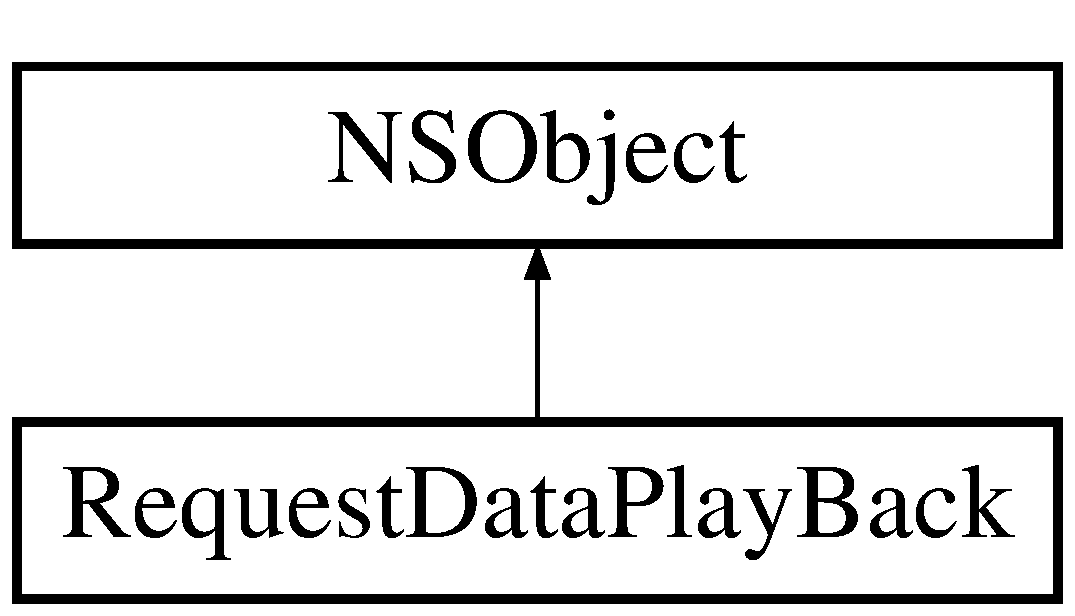
\includegraphics[height=2.000000cm]{interface_request_data_play_back}
\end{center}
\end{figure}
\subsection*{构造函数}
\begin{DoxyCompactItemize}
\item 
(id) -\/ \hyperlink{interface_request_data_play_back_a7684c4a40fb878031fdfb0eff0633316}{init\+Login\+With\+Parameter\+:}
\begin{DoxyCompactList}\small\item\em 登录房间 \end{DoxyCompactList}\item 
(id) -\/ \hyperlink{interface_request_data_play_back_a776ab7183abc45c9ca6c195e1717f29f}{init\+With\+Parameter\+:}
\begin{DoxyCompactList}\small\item\em 进入房间,并请求画图聊天数据并播放视频(可以不登陆,直接从此接口进入直播间) \end{DoxyCompactList}\item 
\mbox{\Hypertarget{interface_request_data_play_back_af780ab6c671e6e4392c40460b1e9312f}\label{interface_request_data_play_back_af780ab6c671e6e4392c40460b1e9312f}} 
(void) -\/ \hyperlink{interface_request_data_play_back_af780ab6c671e6e4392c40460b1e9312f}{request\+Cancel}
\begin{DoxyCompactList}\small\item\em 销毁文档和视频,清除视频和文档的时候需要调用,推出播放页面的时候也需要调用 \end{DoxyCompactList}\item 
\mbox{\Hypertarget{interface_request_data_play_back_aee56b80b39cc622c9621f6c51b8c4ecc}\label{interface_request_data_play_back_aee56b80b39cc622c9621f6c51b8c4ecc}} 
(void) -\/ \hyperlink{interface_request_data_play_back_aee56b80b39cc622c9621f6c51b8c4ecc}{continue\+From\+The\+Time\+:}
\begin{DoxyCompactList}\small\item\em time:从直播开始到现在的秒数,\+S\+D\+K会在画板上绘画出来相应的图形 \end{DoxyCompactList}\item 
\mbox{\Hypertarget{interface_request_data_play_back_ad7e16084e7da421a84e1a45a9cb10fb5}\label{interface_request_data_play_back_ad7e16084e7da421a84e1a45a9cb10fb5}} 
(C\+G\+Float) -\/ \hyperlink{interface_request_data_play_back_ad7e16084e7da421a84e1a45a9cb10fb5}{get\+Doc\+Aspect\+Ratio}
\begin{DoxyCompactList}\small\item\em 获取文档区域内白板或者文档本身的宽高比,返回值即为宽高比,做屏幕适配用 \end{DoxyCompactList}\item 
\mbox{\Hypertarget{interface_request_data_play_back_a3651d4b5f32d770f5542a8f4ee5978ef}\label{interface_request_data_play_back_a3651d4b5f32d770f5542a8f4ee5978ef}} 
(void) -\/ \hyperlink{interface_request_data_play_back_a3651d4b5f32d770f5542a8f4ee5978ef}{change\+Doc\+Frame\+:}
\begin{DoxyCompactList}\small\item\em 改变文档区域大小,主要用在文档生成后改变文档窗口的frame \end{DoxyCompactList}\item 
\mbox{\Hypertarget{interface_request_data_play_back_ac14807bf0739ea6f2f133a643c874bb8}\label{interface_request_data_play_back_ac14807bf0739ea6f2f133a643c874bb8}} 
(void) -\/ \hyperlink{interface_request_data_play_back_ac14807bf0739ea6f2f133a643c874bb8}{change\+Player\+Frame\+:}
\begin{DoxyCompactList}\small\item\em 改变播放器frame \end{DoxyCompactList}\item 
\mbox{\Hypertarget{interface_request_data_play_back_ae205a635e0cad31dde2beec67fae08aa}\label{interface_request_data_play_back_ae205a635e0cad31dde2beec67fae08aa}} 
(void) -\/ \hyperlink{interface_request_data_play_back_ae205a635e0cad31dde2beec67fae08aa}{change\+Player\+Parent\+:}
\begin{DoxyCompactList}\small\item\em 改变播放器父窗口 \end{DoxyCompactList}\item 
\mbox{\Hypertarget{interface_request_data_play_back_a9510f1fefa5e2323763ababc81e30f30}\label{interface_request_data_play_back_a9510f1fefa5e2323763ababc81e30f30}} 
(void) -\/ \hyperlink{interface_request_data_play_back_a9510f1fefa5e2323763ababc81e30f30}{change\+Doc\+Parent\+:}
\begin{DoxyCompactList}\small\item\em 改变文档父窗口 \end{DoxyCompactList}\item 
\mbox{\Hypertarget{interface_request_data_play_back_a79d84970313b229f7081bb5fac4dd623}\label{interface_request_data_play_back_a79d84970313b229f7081bb5fac4dd623}} 
(void) -\/ \hyperlink{interface_request_data_play_back_a79d84970313b229f7081bb5fac4dd623}{pause\+Player}
\begin{DoxyCompactList}\small\item\em 播放器暂停 \end{DoxyCompactList}\item 
\mbox{\Hypertarget{interface_request_data_play_back_a6d244005dfb198942302e23226ada091}\label{interface_request_data_play_back_a6d244005dfb198942302e23226ada091}} 
(void) -\/ \hyperlink{interface_request_data_play_back_a6d244005dfb198942302e23226ada091}{start\+Player}
\begin{DoxyCompactList}\small\item\em 播放器播放 \end{DoxyCompactList}\item 
\mbox{\Hypertarget{interface_request_data_play_back_a3fbf2f0dec509627201b0ff44d1772b7}\label{interface_request_data_play_back_a3fbf2f0dec509627201b0ff44d1772b7}} 
(void) -\/ \hyperlink{interface_request_data_play_back_a3fbf2f0dec509627201b0ff44d1772b7}{shutdown\+Player}
\begin{DoxyCompactList}\small\item\em 播放器关闭 \end{DoxyCompactList}\item 
\mbox{\Hypertarget{interface_request_data_play_back_a1d1e59af956eace4307c70ff4fc8886a}\label{interface_request_data_play_back_a1d1e59af956eace4307c70ff4fc8886a}} 
(void) -\/ \hyperlink{interface_request_data_play_back_a1d1e59af956eace4307c70ff4fc8886a}{stop\+Player}
\begin{DoxyCompactList}\small\item\em 播放器停止 \end{DoxyCompactList}\item 
\mbox{\Hypertarget{interface_request_data_play_back_aba1166b9b5b81faf2d5ad76ac9a856f5}\label{interface_request_data_play_back_aba1166b9b5b81faf2d5ad76ac9a856f5}} 
(void) -\/ \hyperlink{interface_request_data_play_back_aba1166b9b5b81faf2d5ad76ac9a856f5}{replay\+Player}
\begin{DoxyCompactList}\small\item\em 从头重新播放 \end{DoxyCompactList}\item 
\mbox{\Hypertarget{interface_request_data_play_back_a6aabec511ecc8e7ec87128dde263ad07}\label{interface_request_data_play_back_a6aabec511ecc8e7ec87128dde263ad07}} 
(B\+O\+OL) -\/ \hyperlink{interface_request_data_play_back_a6aabec511ecc8e7ec87128dde263ad07}{is\+Playing}
\begin{DoxyCompactList}\small\item\em 播放器是否播放 \end{DoxyCompactList}\item 
\mbox{\Hypertarget{interface_request_data_play_back_a5154fbd4bd4f342a6c260f65ea49501a}\label{interface_request_data_play_back_a5154fbd4bd4f342a6c260f65ea49501a}} 
(N\+S\+Time\+Interval) -\/ \hyperlink{interface_request_data_play_back_a5154fbd4bd4f342a6c260f65ea49501a}{current\+Playback\+Time}
\begin{DoxyCompactList}\small\item\em 播放器当前播放时间 \end{DoxyCompactList}\item 
\mbox{\Hypertarget{interface_request_data_play_back_a3f340787f87e80a56e315b01f5637930}\label{interface_request_data_play_back_a3f340787f87e80a56e315b01f5637930}} 
(void) -\/ \hyperlink{interface_request_data_play_back_a3f340787f87e80a56e315b01f5637930}{set\+Current\+Playback\+Time\+:}
\begin{DoxyCompactList}\small\item\em 设置播放器当前播放时间(用于拖拽进度条时掉用的) \end{DoxyCompactList}\item 
\mbox{\Hypertarget{interface_request_data_play_back_ad1228539b10ec8881a35221ee7d0b734}\label{interface_request_data_play_back_ad1228539b10ec8881a35221ee7d0b734}} 
(N\+S\+Time\+Interval) -\/ \hyperlink{interface_request_data_play_back_ad1228539b10ec8881a35221ee7d0b734}{player\+Duration}
\begin{DoxyCompactList}\small\item\em 回放视频总时长 \end{DoxyCompactList}\item 
\mbox{\Hypertarget{interface_request_data_play_back_aecc0590a3973f70d67a17771e87cf6cd}\label{interface_request_data_play_back_aecc0590a3973f70d67a17771e87cf6cd}} 
(void) -\/ \hyperlink{interface_request_data_play_back_aecc0590a3973f70d67a17771e87cf6cd}{setpause\+In\+Back\+Ground\+:}
\begin{DoxyCompactList}\small\item\em 设置后台是否可播放 \end{DoxyCompactList}\end{DoxyCompactItemize}
\subsection*{属性}
\begin{DoxyCompactItemize}
\item 
\mbox{\Hypertarget{interface_request_data_play_back_a34e93b0b082e759a428100c7db4ab02b}\label{interface_request_data_play_back_a34e93b0b082e759a428100c7db4ab02b}} 
id$<$ Request\+Data\+Play\+Back\+Delegate $>$ \hyperlink{interface_request_data_play_back_a34e93b0b082e759a428100c7db4ab02b}{delegate}
\begin{DoxyCompactList}\small\item\em 代理 \end{DoxyCompactList}\item 
\mbox{\Hypertarget{interface_request_data_play_back_a0e6abb5302bad21cdefb2f41dd183bd3}\label{interface_request_data_play_back_a0e6abb5302bad21cdefb2f41dd183bd3}} 
id$<$ I\+J\+K\+Media\+Playback $>$ \hyperlink{interface_request_data_play_back_a0e6abb5302bad21cdefb2f41dd183bd3}{ijk\+Player}
\begin{DoxyCompactList}\small\item\em 播放器 \end{DoxyCompactList}\end{DoxyCompactItemize}


\subsection{函数文档}
\mbox{\Hypertarget{interface_request_data_play_back_a7684c4a40fb878031fdfb0eff0633316}\label{interface_request_data_play_back_a7684c4a40fb878031fdfb0eff0633316}} 
\index{Request\+Data\+Play\+Back@{Request\+Data\+Play\+Back}!init\+Login\+With\+Parameter\+:@{init\+Login\+With\+Parameter\+:}}
\index{init\+Login\+With\+Parameter\+:@{init\+Login\+With\+Parameter\+:}!Request\+Data\+Play\+Back@{Request\+Data\+Play\+Back}}
\subsubsection{\texorpdfstring{init\+Login\+With\+Parameter\+:()}{initLoginWithParameter:()}}
{\footnotesize\ttfamily -\/ (id) init\+Login\+With\+Parameter\+: \begin{DoxyParamCaption}\item[{(\hyperlink{interface_play_parameter}{Play\+Parameter} $\ast$)}]{parameter }\end{DoxyParamCaption}}



登录房间 


\begin{DoxyParams}{参数}
{\em parameter} & 配置参数信息 必填参数 user\+Id 必填参数 room\+Id 必填参数 liveid 必填参数 viewer\+Name 必填参数 token 必填参数 security \\
\hline
\end{DoxyParams}
\mbox{\Hypertarget{interface_request_data_play_back_a776ab7183abc45c9ca6c195e1717f29f}\label{interface_request_data_play_back_a776ab7183abc45c9ca6c195e1717f29f}} 
\index{Request\+Data\+Play\+Back@{Request\+Data\+Play\+Back}!init\+With\+Parameter\+:@{init\+With\+Parameter\+:}}
\index{init\+With\+Parameter\+:@{init\+With\+Parameter\+:}!Request\+Data\+Play\+Back@{Request\+Data\+Play\+Back}}
\subsubsection{\texorpdfstring{init\+With\+Parameter\+:()}{initWithParameter:()}}
{\footnotesize\ttfamily -\/ (id) init\+With\+Parameter\+: \begin{DoxyParamCaption}\item[{(\hyperlink{interface_play_parameter}{Play\+Parameter} $\ast$)}]{parameter }\end{DoxyParamCaption}}



进入房间,并请求画图聊天数据并播放视频(可以不登陆,直接从此接口进入直播间) 


\begin{DoxyParams}{参数}
{\em parameter} & 配置参数信息 必填参数 user\+Id; 必填参数 room\+Id; 必填参数 liveid; 必填参数 viewer\+Name; 必填参数 token; 必填参数 doc\+Parent; 必填参数 doc\+Frame; 必填参数 player\+Parent; 必填参数 player\+Frame; 必填参数 security; 必填参数 pause\+In\+Back\+Ground; 必填参数 default\+Color; 必填参数 P\+P\+T\+Scaling\+Mode; 必填参数 scaling\+Mode; \\
\hline
\end{DoxyParams}


该类的文档由以下文件生成\+:\begin{DoxyCompactItemize}
\item 
Request\+Data\+Play\+Back.\+h\end{DoxyCompactItemize}

\hypertarget{protocol_request_data_play_back_delegate_01-p}{}\section{$<$Request\+Data\+Play\+Back\+Delegate $>$协议 参考}
\label{protocol_request_data_play_back_delegate_01-p}\index{$<$\+Request\+Data\+Play\+Back\+Delegate $>$@{$<$\+Request\+Data\+Play\+Back\+Delegate $>$}}
类 $<$Request\+Data\+Play\+Back\+Delegate $>$ 继承关系图\+:\begin{figure}[H]
\begin{center}
\leavevmode
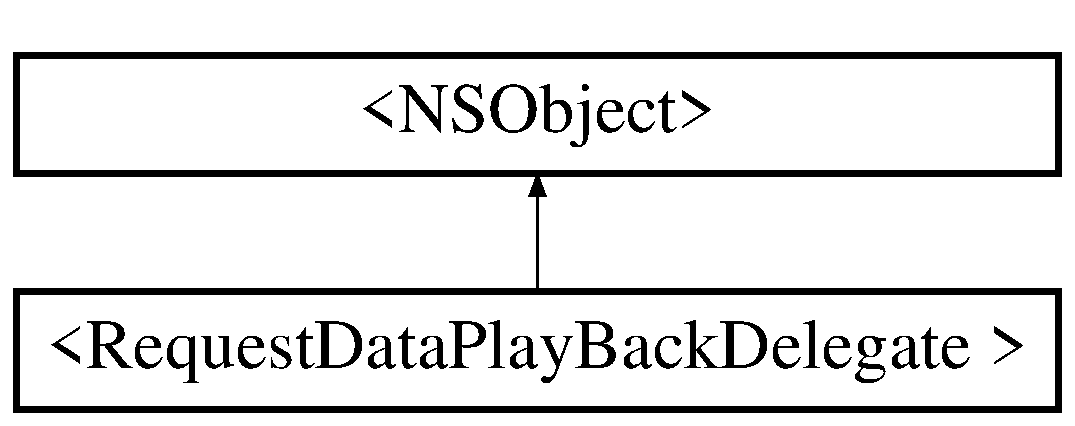
\includegraphics[height=2.000000cm]{protocol_request_data_play_back_delegate_01-p}
\end{center}
\end{figure}
\subsection*{构造函数}
\begin{DoxyCompactItemize}
\item 
\mbox{\Hypertarget{protocol_request_data_play_back_delegate_01-p_a4c6da05d856b8b7dc122a218c31d1bfb}\label{protocol_request_data_play_back_delegate_01-p_a4c6da05d856b8b7dc122a218c31d1bfb}} 
(void) -\/ \hyperlink{protocol_request_data_play_back_delegate_01-p_a4c6da05d856b8b7dc122a218c31d1bfb}{get\+Doc\+Aspect\+Ratio\+Of\+Width\+:height\+:}
\begin{DoxyCompactList}\small\item\em 获取文档内白板或者文档本身的宽高,来进行屏幕适配用的 \end{DoxyCompactList}\item 
\mbox{\Hypertarget{protocol_request_data_play_back_delegate_01-p_aa50c576d7bc5fb8ef7f8d3ef1733aba1}\label{protocol_request_data_play_back_delegate_01-p_aa50c576d7bc5fb8ef7f8d3ef1733aba1}} 
(void) -\/ \hyperlink{protocol_request_data_play_back_delegate_01-p_aa50c576d7bc5fb8ef7f8d3ef1733aba1}{on\+Parser\+Question\+Arr\+:on\+Parser\+Answer\+Arr\+:}
\begin{DoxyCompactList}\small\item\em 收到本房间的历史提问\&回答 \end{DoxyCompactList}\item 
\mbox{\Hypertarget{protocol_request_data_play_back_delegate_01-p_ac1cdee5ae12908f95936f143c58a659d}\label{protocol_request_data_play_back_delegate_01-p_ac1cdee5ae12908f95936f143c58a659d}} 
(void) -\/ \hyperlink{protocol_request_data_play_back_delegate_01-p_ac1cdee5ae12908f95936f143c58a659d}{on\+Parser\+Chat\+:}
\begin{DoxyCompactList}\small\item\em 解析本房间的历史聊天数据 \end{DoxyCompactList}\item 
\mbox{\Hypertarget{protocol_request_data_play_back_delegate_01-p_a9cef2ecbbb3fa09ca031e06cd22982ea}\label{protocol_request_data_play_back_delegate_01-p_a9cef2ecbbb3fa09ca031e06cd22982ea}} 
(void) -\/ \hyperlink{protocol_request_data_play_back_delegate_01-p_a9cef2ecbbb3fa09ca031e06cd22982ea}{request\+Succeed}
\begin{DoxyCompactList}\small\item\em 请求回放地址成功 \end{DoxyCompactList}\item 
\mbox{\Hypertarget{protocol_request_data_play_back_delegate_01-p_a4e89ce484e3ccbaf3c6ba75216101680}\label{protocol_request_data_play_back_delegate_01-p_a4e89ce484e3ccbaf3c6ba75216101680}} 
(void) -\/ \hyperlink{protocol_request_data_play_back_delegate_01-p_a4e89ce484e3ccbaf3c6ba75216101680}{request\+Failed\+:reason\+:}
\begin{DoxyCompactList}\small\item\em 请求回放地址失败 \end{DoxyCompactList}\item 
\mbox{\Hypertarget{protocol_request_data_play_back_delegate_01-p_a77d27553a05331fdb9ac9228caffa8cf}\label{protocol_request_data_play_back_delegate_01-p_a77d27553a05331fdb9ac9228caffa8cf}} 
(void) -\/ \hyperlink{protocol_request_data_play_back_delegate_01-p_a77d27553a05331fdb9ac9228caffa8cf}{login\+Succeed\+Play\+Back}
\begin{DoxyCompactList}\small\item\em 登录成功 \end{DoxyCompactList}\item 
\mbox{\Hypertarget{protocol_request_data_play_back_delegate_01-p_a212a1d84b3c6c7c6912862685bc6c3d2}\label{protocol_request_data_play_back_delegate_01-p_a212a1d84b3c6c7c6912862685bc6c3d2}} 
(void) -\/ \hyperlink{protocol_request_data_play_back_delegate_01-p_a212a1d84b3c6c7c6912862685bc6c3d2}{login\+Failed\+:reason\+:}
\begin{DoxyCompactList}\small\item\em 登录失败 \end{DoxyCompactList}\item 
\mbox{\Hypertarget{protocol_request_data_play_back_delegate_01-p_a5d95b3b010add854c2467f365612d9a3}\label{protocol_request_data_play_back_delegate_01-p_a5d95b3b010add854c2467f365612d9a3}} 
(void) -\/ \hyperlink{protocol_request_data_play_back_delegate_01-p_a5d95b3b010add854c2467f365612d9a3}{room\+Info\+:}
\begin{DoxyCompactList}\small\item\em 获取房间信息,主要是要获取直播间模版来类型,根据直播间模版类型来确定界面布局 房间简介:dic\mbox{[}"desc\char`\"{}\mbox{]};
房间名称:dic\mbox{[}@\char`\"{}name\char`\"{}\mbox{]};
房间模版类型:\mbox{[}dic\mbox{[}@\char`\"{}template\+Type"\mbox{]} integer\+Value\mbox{]}; 模版类型为1\+: 聊天互动: 无 直播文档: 无 直播问答: 无 模版类型为2\+: 聊天互动: 有 直播文档: 无 直播问答: 有 模版类型为3\+: 聊天互动: 有 直播文档: 无 直播问答: 无 模版类型为4\+: 聊天互动: 有 直播文档: 有 直播问答: 无 模版类型为5\+: 聊天互动: 有 直播文档: 有 直播问答: 有 模版类型为6\+: 聊天互动: 无 直播文档: 无 直播问答: 有 \end{DoxyCompactList}\item 
\mbox{\Hypertarget{protocol_request_data_play_back_delegate_01-p_adf21f0ed90eb8d031ee2b8401de592fe}\label{protocol_request_data_play_back_delegate_01-p_adf21f0ed90eb8d031ee2b8401de592fe}} 
(void) -\/ \hyperlink{protocol_request_data_play_back_delegate_01-p_adf21f0ed90eb8d031ee2b8401de592fe}{playback\+\_\+load\+Video\+Fail}
\begin{DoxyCompactList}\small\item\em 加载视频失败 \end{DoxyCompactList}\item 
\mbox{\Hypertarget{protocol_request_data_play_back_delegate_01-p_a4c2ea6e7d5706b8df751e59e63de6f85}\label{protocol_request_data_play_back_delegate_01-p_a4c2ea6e7d5706b8df751e59e63de6f85}} 
(void) -\/ \hyperlink{protocol_request_data_play_back_delegate_01-p_a4c2ea6e7d5706b8df751e59e63de6f85}{page\+Change\+List\+:}
\begin{DoxyCompactList}\small\item\em 回放翻页数据列表 \end{DoxyCompactList}\end{DoxyCompactItemize}


该协议的文档由以下文件生成\+:\begin{DoxyCompactItemize}
\item 
Request\+Data\+Play\+Back.\+h\end{DoxyCompactItemize}

\hypertarget{interface_save_log_util}{}\section{Save\+Log\+Util类 参考}
\label{interface_save_log_util}\index{Save\+Log\+Util@{Save\+Log\+Util}}
类 Save\+Log\+Util 继承关系图\+:\begin{figure}[H]
\begin{center}
\leavevmode
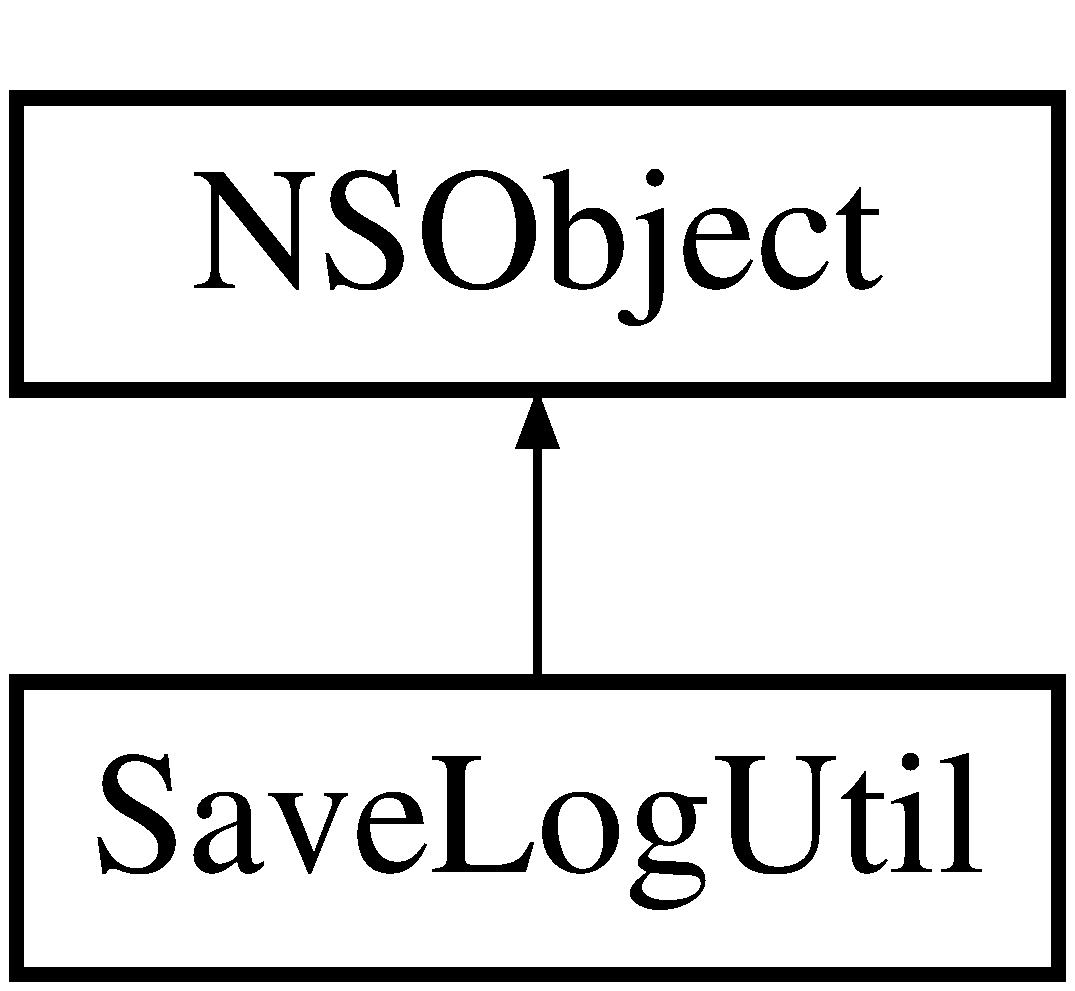
\includegraphics[height=2.000000cm]{interface_save_log_util}
\end{center}
\end{figure}
\subsection*{构造函数}
\begin{DoxyCompactItemize}
\item 
\mbox{\Hypertarget{interface_save_log_util_af6bb7507596eae70afdcaad3a1a0d31e}\label{interface_save_log_util_af6bb7507596eae70afdcaad3a1a0d31e}} 
(void) -\/ \hyperlink{interface_save_log_util_af6bb7507596eae70afdcaad3a1a0d31e}{is\+Need\+To\+Save\+Log\+:}
\begin{DoxyCompactList}\small\item\em 是否需要保存打印 \end{DoxyCompactList}\item 
\mbox{\Hypertarget{interface_save_log_util_ad79d14e9298625ff5308d0122a302f13}\label{interface_save_log_util_ad79d14e9298625ff5308d0122a302f13}} 
(void) -\/ \hyperlink{interface_save_log_util_ad79d14e9298625ff5308d0122a302f13}{save\+Log\+:action\+:}
\begin{DoxyCompactList}\small\item\em 保存打印 \end{DoxyCompactList}\end{DoxyCompactItemize}
\subsection*{类方法}
\begin{DoxyCompactItemize}
\item 
\mbox{\Hypertarget{interface_save_log_util_a4c80ea141f0f85a0e3a457519d0c4a70}\label{interface_save_log_util_a4c80ea141f0f85a0e3a457519d0c4a70}} 
(instancetype) + \hyperlink{interface_save_log_util_a4c80ea141f0f85a0e3a457519d0c4a70}{shared\+Instance}
\begin{DoxyCompactList}\small\item\em 单例 \end{DoxyCompactList}\end{DoxyCompactItemize}


该类的文档由以下文件生成\+:\begin{DoxyCompactItemize}
\item 
Save\+Log\+Util.\+h\end{DoxyCompactItemize}

%--- End generated contents ---

% Index
\backmatter
\newpage
\phantomsection
\clearemptydoublepage
\addcontentsline{toc}{chapter}{索引}
\printindex

\end{document}
